\documentclass{uetgraduation}
\graphicspath{{graph/}}
\begin{document}
\studentname{Hoàng Trung Dũng}
\title{Nghiên cứu phương pháp chống nhiễu cho mạng truyền thông tán xạ ngược sử dụng phương pháp học sâu tăng cường}
\documenttype{Đồ án tốt nghiệp đại học hệ chính quy}
\major{Công nghệ thông tin}
\year{2024}
\supervisor{TS. Nguyễn Ngọc Tân}
\makecovers
% Tóm tắt
\begin{preamble}{Tóm tắt}
\textbf{Tóm tắt:} Truyền thông không dây đã và đang đóng vai trò vô cùng quan trọng trong cuộc sống con người. Tuy
nhiên phương pháp truyền thông này lại rất dễ bị tấn công gây nhiễu do tín hiệu vô tuyến phát sóng trong không gian mở.
Thêm vào đó, với sự phát triển của UAV (thiết bị bay không người lái) với khả năng cung cấp đường truyền tầm nhìn thẳng
(LoS) và hệ số suy giảm đường truyền thấp đã hỗ trợ cho việc tấn công đối với kết nối không dây. Trong khoá luận tốt nghiệp
này, em muốn trình bày một phương án chống nhiễu cho mạng truyền thông không dây, sử dụng học tăng cường sâu, kết hợp với
kỹ thuật tán xạ ngược và thu hoạch năng lượng để không những chống lại mà còn tận dụng được tín hiệu gây nhiễu từ UAV 
để nâng cao hiệu suất của hệ thống truyền thông không dây.

\textit{\textbf{Từ khóa:} Truyền thông không dây, Nhiễu, UAV, Học tăng cường sâu, Tán xạ ngược, Thu năng lượng.}
\end{preamble}
% Lời cảm ơn
\begin{preamble}{Lời cảm ơn}
    Đầu tiên, cho phép em gửi lời cảm ơn đến các thầy, cô giáo trường Đại học Công nghệ - Đại học
    Quốc Gia Hà Nội đã luôn tận tình chỉ bảo và tạo điều kiện trong suốt quá trình em học
    tập tại trường.
    
    Em xin gửi lời cảm ơn sâu sắc đến thầy giáo TS. Nguyễn Ngọc Tân đã tận tình
    hướng dẫn và đóng góp ý kiến quý báu trong suốt quá trình thực hiện khóa luận tốt
    nghiệp của em.
    
    Cuối cùng em xin gửi lời cảm ơn đến gia đình của mình, nơi đã luôn là nguồn động lực cho em
    trong suốt thời gian vừa qua.
    
    Em xin chân thành cảm ơn.
\end{preamble}
% Lời cam đoan
\begin{preamble}{Lời cam đoan}
Tôi xin cam đoan rằng mọi kết quả trình bày trong khóa luận đều do tôi thực hiện
dưới sự hướng dẫn của TS. Nguyễn Ngọc Tân.

Tất cả các tham khảo nghiên cứu liên quan đều nêu rõ nguồn gốc một cách rõ ràng từ 
danh mục tài liệu tham khảo trong khóa luận. Khóa luận không sao chép tài liệu, 
công trình nghiên cứu từ người khác mà không có rõ về mặt tài liệu tham khảo.

Các thông kê, các kết quả trình bày khóa luận đều là tự thực nghiệm khi chạy chương trình. Nếu tôi sai 
tôi hoàn toàn chịu trách nhiệm theo quy định của trường Đại học Công Nghệ - Đại học Quốc Gia Hà Nội.

\begin{flushright}
    Hà Nội, tháng 12 năm 2024

    \vspace{45pt}
    Hoàng Trung Dũng
\end{flushright}
\end{preamble}

% Muc luc
\begin{contentlisting}

\tableofcontents
\listoffigures
% \listoftables

\begin{contentlistingsection}{Các từ viết tắt}
    UAV: unmanned aerial vehicle -- Thiết bị bay không người lái

    LoS: line-of-sight -- Đường truyền tầm nhìn thẳng

    RL: reinforcement learning -- Học tăng cường

    DRL: deep reinforcement learning -- Học tăng cường sâu.
    
    DQN: deep q network -- Mạng sâu Q.

    HTT: harvest then transmit -- Chiến lược thu năng lượng để truyền tin

    RA: rate adaption -- Kĩ thuật điều chỉnh tốc độ phát gói tin

    PSR: packet send ratio -- Tỉ lệ gói tin được máy phát gửi

    PDR: packet delivery ratio -- Tỉ lệ gói tin được gửi thành công đến máy thu

    MAC: medium access control -- Điều khiển truy nhập môi trường

    WLAN: wireless local area network -- Mạng cục bộ không dây

    WSN: wireless sensor network -- Mạng cảm biến không dây

    FHSS: frequency hopping spread spectrum -- Trải phổ nhảy tần

    RA: rate adaption -- Điều chỉnh tốc độ

    RFID: radio frequency identification -- Nhận dạng tần số vô tuyến

    ATG: air-to-ground -- Kênh truyền không đối đất

    MDP: Markov decision process -- Quá trình ra quyết định Markov

    TD: Temporal Difference -- Thuật toán học khác biệt thời gian
\end{contentlistingsection}

\end{contentlisting}

% Chapter 1
\chapter{Đặt vấn đề}
Truyền thông không dây là thành phần không thể thiếu trong cơ sở hạ tầng viễn thông của xã hội ngày nay, có các ứng dụng và
tác động sâu rộng đến mọi mặt của đời sống con người. Mặc dù công nghệ truyền thông không dây đã có rất nhiều bước phát triển
qua nhiều thập kỉ, hầu hết các mạng truyền thông không dây vẫn dễ bị tấn công gây nhiễu bởi tính mở của nó. Bằng cách đưa tín
hiệu nhiễu vào kênh không dây đích, thiết bị gây nhiễu có thể làm giảm tỉ lệ tín hiệu trên nhiễu cộng nhiễu (SINR) của máy thu,
qua đó làm gián đoạn hoặc ngăn chặn kênh truyền không dây hợp lệ. Không giống như những tác động không có chủ đích, tín hiệu gây
nhiễu thường mạnh và qua đó có thể liên tục làm gián đoạn kênh truyền.

Gần đây, thiết bị bay không người lái (UAV) đang ngày càng được sử dụng nhiều hơn để nâng cao năng lực của hạ tầng mạng. Khả năng
triển khai nhanh cùng với tính cơ động cao của UAV khiến nó phù hợp với rất nhiều nhiệm vụ, ví dụ như việc triển khai hệ thống
mạng tạm thời ở những nơi khó tiếp cận như những vùng xảy ra thiên tai, bão lũ... UAV có thể cung cấp đường truyền LoS và hệ số suy
giảm kênh truyền thấp đến người dùng trên mặt đất khi nó được sử dụng như một trạm phát sóng. Do đó UAV có thể được sử dụng để
tăng cường năng lực của hệ thống mạng. Tuy nhiên chính những lợi thế của UAV như ở trên khiến cho nó có thể bị đối tượng xấu 
khai thác như là một thiết bị gây nhiễu di động, ngăn chặn đáng kể việc truyền dữ liệu và làm giảm chất lượng dịch vụ (QoS) của mạng
không dây, nghiêm trọng hơn so với gây nhiễu từ trên mặt đất. Vì thế giải quyết vấn đề gây nhiễu từ UAV là một bài toán đáng quan tâm.

Trong khoá luận này, em sẽ tìm hiểu về tấn công gây nhiễu, cũng như tấn công gây nhiễu từ UAV đối với mạng truyền thông không dây.
Qua đó đề xuất một phương án để không những chống lại mà còn tận dụng cuộc tấn công gây nhiễu để đảm bảo chất lượng đường truyền.
Phần còn lại của khoá luận sẽ được chia thành các chương với nội dung cụ thể như sau:

Chương 2: Cơ sở lý thuyết. Trong chương này trình bày lý thuyết nền tảng về tấn công gây nhiễu và tấn công gây nhiễu bằng UAV.
Cũng như tìm hiểu một số chiến lược chống nhiễu đã được nghiên cứu. Sau đó sẽ đi vào tìm hiểu về RL và DRL - hai phương pháp được
sử dụng để chống nhiễu.

Chương 3: Đề xuất phương án giải quyết bài toán tấn công gây nhiễu từ UAV. Trong chương này, em sẽ mô hình hoá bài toán tấn công
gây nhiễu bằng UAV và đề xuất phương pháp chống nhiễu sử dụng DRL.

Chương 4: Thiết lập mô phỏng và kết quả mô phỏng. Trong chương này, em sẽ trình bày chi tiết về mô hình và thông số thiết lập mô
phỏng phương pháp chống nhiễu được đề xuất. Cũng như so sánh hiệu quả mà phương pháp đề xuất mang lại so với chiến lược phòng thủ
''tham lam''.

Chương 5: Kết luận.

% Chapter 2
\chapter{Cơ sở lý thuyết.}
\section{Mạng không dây.}
\subsection{Giới thiệu.}
Mạng không dây là một hệ thống mạng truyền tải dữ liệu mà không sử dụng các dây cáp kết nối vật lý. Thay vào đó, mạng không dây sử dụng sóng
điện từ để truyền tín hiệu và dữ liệu giữa các thiết bị. Điều này giúp tăng tính di động của thiết bị, vốn là điểm yếu của các kết nối của các
kết nối có dây. Phương pháp gửi dữ liệu thông qua môi trường không khí này được ứng dụng vô cùng sâu rộng trong mọi lĩnh vực đời sống con người
ngày nay, từ công sở, trường học hoặc thậm chí là trong quân sự\dots

Dữ liệu nhận và gửi của mạng không dây được truyền đi xuyên suốt thông qua các tầng ảo sau:
\begin{itemize}
    \item Tầng vật lý: Là tầng thể hiện đặc điểm của kết nối vật lý giữa các thiết bị trong mạng, trong trường hợp mạng không dây, môi trường truyền
    là không khí. Quá trình nhận và truyền dữ liệu được quản lý bởi tầng vật lý. Trong mạng không dây, dữ liệu nhị phân giữa các thiết bị được chuyển
    thành tín hiệu điện và sử dụng tần số vô tuyến để gửi và nhận dữ liệu, tất cả quá trình này được thực hiện bởi tầng vật lý. Đây cũng là tầng chịu
    thiệt hại nặng nề nhất từ cuộc tấn công gây nhiễu sóng vô tuyến.
    \item Tầng liên kết dữ liệu: Là tầng ở giữa, chịu trách nhiệm kết nối giữa tầng vật lý và tầng mạng, ngoài ra còn thực hiện phân đoạn các gói được
    gửi bởi các tầng cao hơn thành các khung có thể được gửi bởi tầng vật lý. Tầng này cũng cung cấp khả năng kiểm tra lỗi và định dạng các khung dữ liệu
    được gửi. Tầng con MAC của tầng liên kết dữ liệu chịu trách nhiệm di chuyển các gói dữ liệu đến và đi từ nút này sang nút khác trên một kênh chung.
    Kênh truyền trong mạng không dây là một tần số mà các nút sử dụng để gửi dữ liệu. Tầng con MAC sử dụng giao thức MAC để đảm bảo tín hiệu gửi từ các
    trạm khác nhau trên cùng một kênh truyền không bị xung đột. Tầng này dễ bị tấn công gây nhiễu tầng liên kết dữ liệu - các thiết bị gây nhiễu tinh vi
    có thể tận dụng lợi thế của tầng liên kết dữ liệu và tạo ra cuộc tấn công hiệu quả về mặt năng lượng. So với tấn công gây nhiễu sóng vô tuyến ở tầng
    vật lý, gây nhiễu tầng liên kết dữ liệu tối ưu hơn về mặt năng lượng.
    \item Tầng mạng: Hoạt động như một liên kết giữa tầng giao vận ở trên và tầng liên kết dữ liệu ở dưới. Chịu trách nhiệm tìm ra cấu trúc mạng và gán địa
    chỉ, cũng như định tuyến dữ liệu.
    \item Tầng giao vận: Khôi phục dữ liệu bị mất và cũng chịu trách nhiệm truyền lại dữ liệu. Cung cấp khả năng mã hoá dữ liệu và truyền dữ liệu đáng tin cậy.
    \item Tầng ứng dụng: Tầng này chịu trách nhiệm xác định thông số kỹ thuật của dữ liệu được yêu cầu bởi cả người dùng cuối cũng như các nút trong mạng. 
\end{itemize}

\subsection{Phân loại mạng không dây và ứng dụng.}
\begin{itemize}
    \item WLAN: mạng không dây cục bộ, hay còn được biết đến nhiều hơn là Wi-Fi. WLAN cho phép thiết bị kết nối với Internet dễ dàng miễn là nó được kết nối với
    sóng Wi-Fi. WLAN được sử dụng ở rất nhiều nơi xung quanh chúng ta ngày nay, từ hộ gia đình, trường học, công sở, địa điểm kinh doanh\dots Thiết bị di động
    kết nối với điểm truy cập thông qua kết nối không dây sẽ có thể kết nối Internet và di chuyển một cách tự do, miễn là thiết bị đó ở trong tầm phủ sóng của
    sóng Wi-Fi.

    Hình 2.1 mô tả một mạng không dây cục bộ với một điểm truy cập và bốn thiết bị kết nối thông qua môi trường không dây.
    \begin{figure}{Mạng không dây cục bộ.}
        \centering
        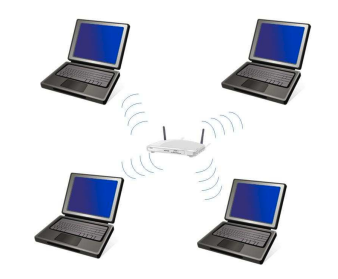
\includegraphics[scale=0.6]{wlan}
        \label{fig:wlan}
    \end{figure}
    \item WSN: Mạng cảm biến không dây, là một tập hợp số lượng lớn các nút có khả năng thu thập dữ liệu từ môi trường xung quanh và truyền tải thông tin
    về trung tâm xử lý dữ liệu hoặc các thiết bị thu thập dữ liệu. Trong WSN, các nút có thể chia sẻ thông tin cho nhau, dữ liệu thu thập từ các cảm biến không được
    gửi trực tiếp cho người dùng mà được xử lý và tổng hợp lại, chỉ gửi những thông tin mục tiêu mà mạng cảm biến muốn đạt được. Do đó những dữ liệu tạm thời, không
    cần thiết, chưa qua xử lý hoặc dữ liệu trung gian giữa các nút sẽ không được gửi tới người dùng.
    \begin{figure}{Mạng cảm biến không dây.}
        \centering
        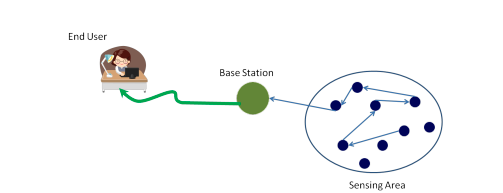
\includegraphics[scale=0.6]{wsn}
        \label{fig:wsn}
    \end{figure}

    Mạng cảm biến không dây có một số ứng dụng sau:
    \begin{itemize}
        \item Sử dụng trong lĩnh vực an ninh như giám sát ở các khu vực nhạy cảm để phát hiện các mối đe doạ như tấn công sinh học hoặc hoá học\dots
        \item Giám sát môi trường: WSN hỗ trợ thu thập thông tin ở những khu vực khó thiết lập cơ sở hạ tầng để giám sát môi trường cũng như môi trường sống.
        \item Trong y học: sử dụng để giúp các bác sĩ theo dõi sức khoẻ của bệnh nhân.
        \item Theo dõi đối tượng: WSN có thể dùng để theo dõi các đối tượng chuyển động nếu sử dụng cảm biến phù hợp.
        \item Hỗ trợ người khuyết tật: Người khuyết tật có thể độc lập hơn và cải thiện khả năng hoạt động với việc sử dụng WSN, WSN cho phép tự chăm sóc hiệu
        quả hơn và nâng cao chất lượng cuộc sống.
    \end{itemize}

    \item Mạng không dây tạm thời (ad hoc): là mạng không dây không cần bất kì cơ sở hạ tầng hiện có nào để triển khai ví dụ như điểm truy cập hoặc dây cáp.
    Mỗi thiết bị trong mạng coi là một nút tham gia trực tiếp vào việc định tuyến dữ liệu một cách độc lập bằng cách chuyển tiếp dữ liệu từ nút này sang nút khác
    mà không cần thêm bất kì một thiết bị quản lý tập trung nào như điểm truy cập\dots Mỗi nút trong mạng không dây tạm thời tự động quyết định nút nào sẽ gửi dữ
    liệu tiếp theo tuỳ thuộc vào kết nối mạng. Hình 2.3 là một mô hình đơn giản của mạng không dây tạm thời giữa các thiết bị kết nối với nhau mà không có điểm
    truy cập nào.
    \begin{figure}{Mạng không dây tạm thời.}
        \centering
        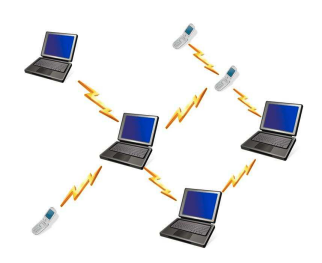
\includegraphics[scale=0.6]{ad_hoc}
        \label{fig:adhoc}
    \end{figure}

    Ứng dụng của mạng không dây tạm thời:
    \begin{itemize}
        \item Trong quân sự: người lính, các thiết bị quân sự như xe tăng, tàu chiến có thể kết nối với nhau mà không cần một cơ sở hạ tầng mạng không dây rõ ràng
        bằng cách hình thành một mạng không dây tạm thời.
        \item Mạng không dây tạm thời có thể được sử dụng trong các nhiệm vụ thực thi pháp luật, giải cứu\dots
        \item Có thể được sử dụng trong hội nghị, cuộc họp, bài giảng hoặc các khu vực phục vụ mục đích thương mại, nơi tải mạng có thể rất cao.
    \end{itemize}
\end{itemize}


\section{Tấn công gây nhiễu sóng vô tuyến.}
Trong mạng truyền thông không dây, đặc tính mở của môi trường truyền, cụ thể ở đây mạng không dây sử dụng không khí là môi trường truyền để truyền và nhận dữ
liệu, dẫn đến việc nó rất dễ bị tấn công bởi nhiều kiểu tấn công khác nhau. Ở đây chúng ta nghiên cứu cụ thể loại tấn công mạng không dây bằng gây nhiễu sóng
vô tuyến.

\subsection{Giới thiệu.}
Tấn công gây nhiễu sóng vô tuyến được định nghĩa là một hành động cố tình can thiệp vào quá trình truyền và nhận vật lý của truyền thông
không dây. Trong đó kẻ tấn công (máy gây nhiễu) sẽ phát tín hiệu vô tuyến trên cùng băng tần mà mạng mục tiêu sử dụng. Mục tiêu của việc
tấn công là làm giảm hiệu suất mạng hoặc thậm chí ngăn chặn hoàn toàn việc truyền thông tin không dây giữa các thiết bị.

Trong cuộc tấn công gây nhiễu, máy gây nhiễu đưa năng lượng gây nhiễu vào môi trường không dây, gây cản trở việc truyền tải hợp pháp theo
một trong hai cách: 
\begin{itemize}
    \item Máy gây nhiễu gửi tín hiệu nhiễu mạnh gây giảm tỉ lệ tín hiệu trên nhiễu cộng với nhiễu (SINR) ở máy thu.
    \item Gây nhiễu liên tục ngăn cản việc máy phát truy cập vào kênh truyền, dẫn đến một cuộc tấn công từ chối dịch vụ (DOS). Tấn công từ
    chối dịch vụ thực hiện bằng cách gửi tín hiệu nhiễu, gói tin giả khiến kênh truyền hợp lệ bận, làm cho máy phát ngừng gửi bất kì dữ liệu nào
    cho đến khi kênh truyền khả dụng trở lại.
\end{itemize}

Tấn công gây nhiễu sóng vô tuyến có một số đặc điểm sau đây:
\begin{itemize}
    \item Cố ý: Đây là hành động gây nhiễu có chủ đích của kẻ tấn công, nhằm vào một mục tiêu cụ thể, không giống với nhiễu tự nhiên gây
    ra bởi các yếu tố của môi trường.
    \item Không tuân thủ các giao thức MAC: đặc điểm chung của các cuộc tấn công gây nhiễu là việc liên lạc của chúng không tuân theo các
    giao thức MAC.
    \item Phạm vi tấn công: Máy gây nhiễu có thể nhắm vào một tần số cố định hoặc nhiều tần số khác nhau.
\end{itemize}

\subsection{Thông số đánh giá một cuộc tấn công gây nhiễu.}
Trong tấn công gây nhiễu sóng vô tuyến, các thông số sau phản ánh tác động của cuộc tấn công đến mạng không dây.
\begin{itemize}
    \item \textbf{SINR}: tỉ lệ tín hiệu trên nhiễu cộng nhiễu là tỉ số giữa công suất của tín hiệu máy phát so với tín hiệu gây nhiễu như
    tín hiệu từ máy gây nhiễu và nhiễu môi trường trong kênh truyền
    \[
    \theta = \frac{P_R}{\varphi P_J + \rho^2}
    \]
    Trong đó $P_R$ là công suất nhận được từ máy phát tại cổng (máy thu), $P_J$ là công suất nhiễu được phát của máy gây nhiễu, $\rho^2$ là phương sai
    của nhiễu Gauss trắng cộng thêm. $\varphi P_J$ là công suất nhiễu tại cổng, trong đó $0 \leq \varphi \leq 1$ là hệ số suy giảm kênh truyền.

    Có thể thấy tín hiệu nhiễu càng mạng càng làm giảm giá trị SINR ở máy thu, khiến cho tỉ lệ lỗi bit (BER) tăng, gây lỗi khi giải mã gói tin ở máy thu,
    làm giảm thông lượng và độ tin cậy của kết nối giữa máy phát và máy thu.
    \item \textbf{Thông lượng}: được định nghĩa là tốc độ trung bình gửi gói tin thành công thông qua kênh truyền, được tính thông qua công thức Shannon:
    \[
    C = B \log_2(1 + \text{SINR})
    \]
    Trong đó $C$ là dung lượng kênh hoặc thông lượng lý thuyết tối đa (bit/s), B là băng thông của kênh (Hz). Ta có thể nhận thấy thông qua công thức này,
    thông lượng của kênh giảm khi có sự xuất hiện của tín hiệu gây nhiễu làm giảm chỉ số SINR.
    \item \textbf{PSR}: đại diện cho tỉ lệ giữa gói tin thực sự được gửi thành công bởi máy phát và số gói tin mà máy phát dự định gửi. Nếu máy phát có ý
    định gửi n gói tin và máy thu chỉ nhận được m gói tin ($m \leq n$) thì PSR được tính như sau:
    \[
    PSR = \frac{m}{n}
    \]
    Số gói tin bị mất so với gói tin dự định gửi là do nhiễu. Tín hiệu nhiễu khiến cho kênh truyền luôn bận khiến máy phát không thể truyền gói tin đến máy
    thu, dẫn đến gói tin mới đến máy phát bị loại bỏ do hàng đợi gói tin của máy phát đầy, hoặc gói tin bị loại do ở quá lâu trong hàng đợi. Các giao thức
    MAC khác nhau có cách xác định kênh truyền đang bận hay không khác nhau, một trong số đó là nếu cường độ tín hiệu của kênh lớn hơn ngưỡng xác định trước,
    kênh sẽ được xác định là bận.
    \item \textbf{PDR}: là tỉ lệ số gói tin được gửi thành công đến máy thu so với số gói tin được máy phát gửi đi. Sau khi gói tin được máy phát gửi, máy thu
    vẫn có thể không giải mã được gói tin do ảnh hưởng của nhiễu, dẫn đến gói tin gửi không thành công. PDR có thể được tính ở máy thu bằng tỉ lệ giữa số gói
    tin nhận được và số gói tin vượt qua được kiểm tra CRC - là kĩ thuật phát hiện lỗi thường được dùng trong mạng truyền thông.
    
    Giả sử n là số gói tin máy thu nhận được và q là số gói tin vượt qua kiểm tra CRC thì:
    \[
    PDR = \frac{q}{n}
    \]
    Ngoài ra PDR còn có thể được tính ở máy phát bằng số gói tin ACK mà máy phát nhận được từ máy thu. Trong cả 2 trường hợp, nếu không có gói tin nào nhận thành
    công ở máy thu, PDR được xác định là 0.
\end{itemize}


\subsection{Các mô hình tấn công gây nhiễu.}
Có rất nhiều chiến lược tấn công khác nhau mà máy gây nhiễu có thể thực hiện để làm nhiễu mạng không dây. Do đó cũng dẫn đến nhiều mô hình tấn công với
nhiều mức độ hiệu quả khác nhau. Tuy nhiên sau đây là một số mô hình gây nhiễu đã chứng minh được tính hiệu quả trong việc làm gián đoạn kết nối mạng không
dây.
\begin{itemize}
    \item \textbf{Máy gây nhiễu liên tục}: thiết bị gây nhiễu liên tục phát ra tín hiệu vô tuyến mà không có sự gián đoạn. Tín hiệu nhiễu phát ra có thể 
    là sóng điện từ đơn giản hoặc thậm chí là các bit dữ liệu. Sóng điện từ hoặc các bit dữ liệu được máy gây nhiễu phát ra này không tuân theo bất kì giao 
    thức hoặc quy tắc nào mà các nút trong mạng tuân theo. Kiểu máy gây nhiễu này làm giảm PDR bằng cách làm hỏng các bit tại máy thu, khiến máy thu không
    thể giải mã dữ liệu. Nó cũng có thể làm giảm PSR bằng cách giữ cho kênh truyền giữa máy phát và máy thu liên tục bận, ngăn chặn việc máy phát truyền sử
    dụng đường truyền hợp lệ để truyền gói tin đến máy thu.
    \item \textbf{Máy gây nhiễu lừa đảo}: loại máy gây nhiễu này rất giống với máy gây nhiễu liên tục do cùng liên tục truyền tín hiệu hoặc dữ liệu qua mạng.
    Tuy nhiên điểm khác biệt là máy gây nhiễu lừa đảo không truyền các bit dữ liệu ngẫu nhiên. Máy gây nhiễu giả mạo liên tục đưa các gói tin vào mạng mà không
    có bất kì khoảng cách nào giữa các lần truyền, và do dữ liệu không phải là các bit ngẫu nhiên, do đó khiến cho nút mạng tin rằng những bit dữ liệu này là
    hợp lệ và do đó không sử dụng đường truyền nữa. Ví dụ máy gây nhiễu có thể gửi gói tin ACK giả mạo để khiến máy phát tin rằng nó đã truyền dữ liệu thành công.
    \item \textbf{Máy gây nhiễu ngẫu nhiên}: hai kiểu máy gây nhiễu ở trên luôn luôn duy trì việc truyền tín hiệu hoặc dữ liệu vào mạng, dẫn đến việc nó không
    hiệu quả về mặt năng lượng và phải kết nối với nguồn năng lượng bên ngoài khiến nó hạn chế khả năng di chuyển. Máy gây nhiễu ngẫu nhiên mặt khác có chu kỳ ngủ
    và chu kỳ gây nhiễu, cả hai chu kỳ có thể tuân theo một phân phối xác suất hoặc có thể hoàn toàn là ngẫu nhiên. Việc có cả hai trạng thái ngủ và gây nhiễu
    khiến máy gây nhiễu có thể tắt tín hiệu gây nhiễu qua đó tiết kiệm năng lượng trong giai đoạn ngủ và hoạt động như bất kỳ máy gây nhiễu nào trong hai máy gây 
    nhiễu đã thảo luận ở trên trong chu kỳ gây nhiễu của nó.
    \item \textbf{Máy gây nhiễu phản ứng}: ba mô hình gây nhiễu ở trên là ba mô hình gây nhiễu chủ động theo nghĩa là chúng luôn chủ động tấn công kênh truyền
    bất kể lưu lượng qua kênh như thế nào. Gây nhiễu chủ động thường hiệu quả vì chúng khiến kênh truyền luôn bận rộn, tuy nhiên lại có nhược điểm là dễ bị phát
    hiện. Một cách tiếp cận khác so với gây nhiễu chủ động là gây nhiễu phản ứng, tức là không cần thiết phải tấn công kênh truyền khi không có lưu lượng trên đường
    truyền. Thay vào đó máy gây nhiễu phản ứng sẽ không hoạt động khi kênh truyền rảnh rỗi, và bắt đầu phát tín hiệu gây nhiễu ngay khi nó cảm nhận được hoạt động
    truyền phát tín hiệu trên kênh. Do đó nó nhắm vào việc nhận tin nhắn. Thiết bị gây nhiễu phản ứng có thể không tối ưu về mặt năng lượng do nó phải liên tục lắng
    nghe để cảm nhận kênh truyền. Tuy nhiên nó khó bị phát hiện hơn gây nhiễu chủ động.
\end{itemize}

\section{Tấn công gây nhiễu bằng UAV.}
Trong phần này, chúng ta cùng xem xét về mô hình kênh truyền ATG giữa UAV và thiết bị trên mặt đất, qua đó đưa ra một số cơ sở lý thuyết về bài toán tấn công gây
nhiễu bằng UAV.

Xem xét một UAV gây nhiễu, thiết bị I nằm trên mặt đất chịu tác động của tín hiệu nhiễu UAV, kênh liên lạc giữa UAV và thiết bị I được mô 
hình hoá là kênh không đối đất ATG, bao gồm ba thành phần là:
\begin{itemize}
    \item Đường truyền tầm nhìn thẳng LoS: không có vật cản giữa UAV và thiết bị
    \item Đường truyền không tầm nhìn thẳng NLoS: tín hiệu không thể đi thẳng giữa UAV và thiết bị vì có vật cản như cây cối, toà nhà, địa hình\dots 
    \item Pha đinh quy mô nhỏ (small-scale fading): là sự biến động tín hiệu nhanh chóng do hiện tượng đa đường, gây ra các thay đổi về cường độ tín hiệu khi môi trường
    thay đổi\dots
\end{itemize}

Về cơ bản, tác động của pha đinh quy mô nhỏ nhỏ hơn nhiều so với LoS và NLoS, do đó yếu tố này bị bỏ qua. Suy hao đường truyền của kênh không đối đất giữa UAV và thiết
bị I được tính như sau:
\begin{align*}
    PL &= \begin{cases}
        \beta_\text{LoS}|d|^{-\alpha}, & \text{với đường truyền LoS} \\
        \beta_\text{NLoS}|d|^{-\alpha}, & \text{với đường truyền NLoS} \\
    \end{cases}
\end{align*}

Trong đó $\beta_\text{LoS}$ và $\beta_\text{NLoS}$ lần lượt là hệ số suy giảm bổ sung của kênh truyền LoS và NLoS, $d$ là khoảng cách giữa UAV và thiết bị I,
$\alpha$ là hệ số suy hao đường truyền của kênh ATG. 

Xác suất của kết nối LoS, phụ thuộc vào góc nâng $\theta_i$ giữa thiết bị I và UAV, môi trường truyền thông, mật độ xây dựng xung quanh và chiều cao $H_J$ của UAV,
có thể được biểu diễn như sau:
\[
P_\text{LoS} = \frac{1}{1 + \Phi \exp(-\Psi [\theta_i - \Phi])}
\]
Trong đó $\Phi$ và $\Psi$ là các tham số của đường cong chữ S, phụ thuộc vào môi trường truyền, ví dụ $\Phi = 150$ và $\Psi =15$ là các giá trị thường được sử dụng trong
môi trường đô thị, góc $\theta_i$ được tính như sau:
\[
\theta_i = \frac{180}{\pi} \arcsin(\frac{H_J}{d})
\]

Xác suất của kết nối NLoS là $P_\text{NLoS} = 1 - P_\text{LoS}$. Do đó giá trị kì vọng của công suất nhiễu của UAV gây ra ở thiết bị I là:
\[
P_\text{Ji} = P_J P_\text{LoS} \beta_\text{LoS} |d|^{-\alpha} + P_J P_\text{NLoS} \beta_\text{NLoS} |d|^{-\alpha}
\]
Trong đó $P_J$ là công suất của UAV gây nhiễu.

Do đó khi UAV di chuyển, khoảng cách $d$ và góc nâng $\theta_i$ giữa UAV và thiết bị i thay đổi, dẫn đến sự thay đổi cường độ nhiễu tại thiết bị I.
Điều này khiến cho tác động của nhiễu UAV lên thiết bị I thay đổi do tỉ lệ tín hiệu trên nhiễu cộng nhiễu SINR thay đổi.


\section{Kỹ thuật chống nhiễu.}
Có nhiều biện pháp đối phó khác nhau để ngăn chặn và giảm thiểu tác động của các cuộc tấn công gây nhiễu, sau đây là một số biện pháp.

\subsection{Điều chỉnh công suất phát.}
Đây là cách tiếp cận đơn giản và phổ biến nhất, cụ thể máy phát có thể quyết định phát ở mức công suất thấp để khiến máy gây nhiễu khó khăn hơn trong việc phát hiện
tín hiệu truyền phát. Cách tiếp cận này chỉ khả thi trong việc đối phó với máy gây nhiễu phản ứng và khiến hiệu suất truyền tải giảm xuống rõ rệt. Ngoài ra máy phát
có thể lựa chọn tăng công suất phát để lấn át tín hiệu nhiễu ở máy thu, tuy nhiên cách này tốn nhiều năng lượng và không hiệu quả nếu máy gây nhiễu tấn công với mức
năng lượng rất lớn.

\subsection{Trải phổ nhảy tần - FHSS.}
Trải phổ là kĩ thuật điều chế giúp trải rộng dữ liệu trên toàn bộ băng tần, mặc dù không cần toàn bộ băng tần để gửi dữ liệu đó. Việc trải rộng dữ liệu vượt quá giới
hạn cần thiết trên toàn bộ băng tần giúp cho tín hiệu có khả năng chống lại nhiễu.

FHSS là một kĩ thuật trải phổ, trong đó tín hiệu phát chuyển đổi nhanh chóng giữa các kênh tần số. Việc thay đổi kênh được thực hiện bằng thuật toán được chia sẻ giữa
máy phát và máy thu trước khi trao đổi dữ liệu. Khi kênh hiện tại bị tấn công, máy phát có thể chuyển sang kênh liên lạc khác để truyền dữ liệu. Nhiều chiến lược tối
ưu khác nhau nhằm tối đa hoá thông lượng có thể được sử dụng để máy phát chọn tần số để nhảy khi bị tấn công gây nhiễu như học Q hoặc học sâu Q, hoặc áp dụng lý thuyết
trò chơi\dots Tuy nhiên điểm yếu của FHSS là kĩ thuật này đòi hỏi nhiều tài nguyên phổ tần hơn để nhảy tần và tránh máy gây nhiễu, nếu máy gây nhiễu đủ mạnh để tấn công
nhiều kênh truyền đồng thời thì FHSS trở nên kém hiệu quả hơn.

\subsection{Kĩ thuật điều chỉnh tốc độ - Kĩ thuật RA.}
Kĩ thuật điều chỉnh tốc độ cung cấp một cơ chế quan trọng cho hệ thống không dây đánh đổi giữa tốc độ dữ liệu ở tầng vật lý và độ bền vững của hệ thống (khả năng duy
trì hiệu suất và độ ổn định của mạng ngay cả trong môi trường bất lợi) nhằm tối đa hoá hiệu suất. RA được coi là cơ chế của tầng MAC và nhiều giải thuật điều chỉnh
tốc độ được nghiên cứu, hầu hết dựa trên thông tin của tầng MAC, ví dụ như lựa chọn tốc độ phát dựa trên số khung bị mất. Giả thiết là khi số khung bị mất tăng lên,
có nghĩa là kênh truyền đang suy giảm chất lượng, và máy phát nên giảm tốc độ dữ liệu vật lý bằng cách sử dụng sơ đồ điều chế hoặc mã hoá mạnh mẽ hơn. Tuy nhiên trong
trường hợp khung bị mất do nhiễu thay vì suy giảm kênh, việc giảm tốc độ truyền có thể thậm chí gây ra tỉ lệ mất mát cao hơn do kéo dài thời gian truyền của khung.

Trong môi trường bị tấn công, ý tưởng chính của kĩ thuật RA là chủ động hoặc thích ứng điều chỉnh tốc độ phát xuống mức thấp hơn. Về cơ bản, RA sử dụng thuật toán điều 
chỉnh tốc độ để lựa chọn tốc độ phát phù hợp dựa trên điều kiện hiện tại của kênh. Do đó, RA có thể giúp tăng độ tin cậy của đường truyền và vẫn cung cấp thông lượng 
trên kênh trong trường hợp bị nhiễu tấn công. Tuy nhiên, một số nghiên cứu đã chỉ ra rằng kĩ thuật RA không hiệu quả trên một kênh đơn, và nó cũng không hiệu
quả để đối phó với một cuộc tấn công thông minh.

\section{Tán xạ ngược môi trường xung quanh.}
\subsection{Giới thiệu.}
Tán xạ ngược môi trường xung quanh là một kĩ thuật truyền thông cho phép hai thiết bị có thể truyền dữ liệu cho nhau nhờ việc tận dụng tín hiệu tần số vô tuyến từ môi trường 
xung quanh. Tín hiệu môi trường xung quanh là những tín hiệu có sẵn trong môi trường như tín hiệu nhiễu, tín hiệu truyền hình, tín hiệu di động.

So với liên lạc vô tuyến truyền thống, kĩ thuật tán xạ ngược này cho phép truyền thông tin mà không cần các quá trình tiêu hao nhiều năng lượng như tạo ra sóng vô tuyến, 
do đó nó có mức độ tiết kiệm năng lượng cao hơn. 

So với kĩ thuật tán xạ ngược truyền thống, ví dụ như RFID hoạt động theo nguyên lý sau: đầu đọc RFID sẽ truyền các tín hiệu công suất cao (1W) đến 
các thiết bị lân cận như thẻ RFID thụ động - không có pin và hoạt động dựa trên việc thu năng lương từ tín hiệu của đầu đọc RFID, sau đó tán xạ tín hiệu này để gửi thông tin
đến đầu đọc RFID, đầu đọc sau đó sẽ giải mã tín hiệu tán xạ này để trích xuất dữ liệu. So với kĩ thuật RFID này thì tán xạ ngược môi trường xung quanh có một số điểm ưu việt hơn.
Thứ nhất, do tận dụng tín hiệu trong môi trường nên nó không cần phải có thêm cơ sở hạ tầng cung cấp năng lượng như đầu đọc RFID cung cấp năng lượng cho các thiết bị lân cận 
thông qua việc phát tín hiệu công suất cao. Điều này giúp giảm chi phí lắp đặt và bảo trì, thứ khiến cho hệ thống như RFID khó khăn nếu triển khai ở những môi trường ngoài trời
hoặc trải rộng trên một không gian rộng lớn. Thứ hai, tác động của nó với môi trường rất nhỏ do nó không tiêu thụ thêm nguồn năng lượng nào ngoài năng lượng có sẵn trong không
khí. Cuối cùng nó cung cấp khả năng liên lạc trực tiếp giữa các thiết bị, không giống như hệ thống RFID mà các thẻ cần giao tiếp riêng với đầu đọc và không thể cảm nhận được sự
truyền tải của các thẻ lân cận.

\subsection{Mô tả nguyên lý hoạt động.}
\begin{enumerate}
    \item [\textbf{a.}] \textbf{Quá trình truyền gói tin ở máy phát.}
    
    Thiết kế của máy phát trong tán xạ ngược môi trường xung quanh dựa trên kĩ thuật truyền thông tán xạ ngược thông thường. Về cơ bản, tán xạ ngược đạt được bằng cách thay đổi
    trở kháng của ăng ten. Theo trực giác, khi sóng gặp ranh giới giữa hai môi trường có trở kháng hoặc mật độ khác nhau thì sóng bị phản xạ trở lại. Điều này đúng trong cho dù
    là trong trường hợp sóng cơ truyền qua một sợi dây treo vào một điểm cố định trên tường hay sóng điện từ khi gặp ăng ten. Bằng cách điều chỉnh trở kháng của ăng ten, người ta
    có thể điều chỉnh năng lượng sóng RF đến bị tán xạ, từ đó cho phép truyền thông tin. Máy phát sẽ điều chế và phản xạ tín hiệu vô tuyến xung quanh hoặc tín hiệu gây nhiễu bằng
    cách sử dụng bộ điều biến tải. Đầu vào của bộ điều biến tải là một chuỗi các bit 0,1 được tạo ra dựa theo gói tin, khi bit đầu vào là 0, bộ điều biến tải thay đổi trở kháng
    thành $Z_1$ và do đó máy phát ở trạng thái không phản xạ. Khi bit đầu vào là 1, bộ điều biến tải thay đổi trở kháng thành $Z_2$ qua đó máy phát ở trạng thái phản xạ. Bằng cách
    này, máy phát có thể tán xạ ngược gói tin đến máy thu. Lưu ý là trong khi thực hiện tán xạ ngược, máy phát còn có thể thu năng lượng (ở trạng thái không phản xạ) nhưng lượng
    năng lượng thu được là tương đối nhỏ và chỉ đủ dùng cho các hoạt động của mạch tán xạ ngược.
    
    \item [\textbf{b.}] \textbf{Quá trình giải mã gói tin ở máy thu.}
    
    Để máy thu có thể giải mã tín hiệu tán xạ ngược thông tin với tốc độ thấp hơn tín hiệu môi trường xung quanh (cụ thể là tín hiệu gây nhiễu và tín hiệu môi trường xung quanh).
    Quá trình giải mã có thể được mô tả như sau. Giả sử chúng ta có một bộ thu kĩ thuật số lấy mẫu tín hiệu ở tốc độ thông tin Nyquist (giả sử dùng ADC), tín hiệu nhận được ở máy thu được lấy mẫu
    thành $y[n]$ như sau:
    \[
    y[n] = x[n] + \alpha B[n]x[n] + w[n]
    \]
    Trong đó $x[n]$ là mẫu của tín hiệu môi trường xung quanh (có thể là tín hiệu gây nhiễu) nhận được ở máy thu, $w[n]$ là nhiễu môi trường, $\alpha$ là sự suy giảm phức tạp của
    tín hiệu tán xạ ngược, $B[n]$ là các bit dữ liệu được truyền bởi máy phát. Nếu máy phát truyền thông tin với tốc độ một phần nhỏ, giả sử là $\frac{1}{N}$ dẫn đến $B[Ni + j]$ bằng
    nhau với j = 1 đến N. Sau đó máy thu tính công suất trung bình của N mẫu nhận được như sau:
    \[
    \frac{1}{N}\sum_{i=1}^N|y[n]|^2 = \frac{1}{N}\sum_{i=1}^N|x[n] + \alpha B x[n] + w[n]|^2
    \]
    Với B nhận giá trị 0 hoặc 1 tuỳ thuộc vào trạng thái không phản xạ hoặc phản xạ. Do $x[n]$ không tương quan với nhiễu $w[n]$ nên công thức bên trên có thể được viết lại như sau;
    \[
    \frac{1}{N} \sum_{i=1}^{N}|y[n]|^2 = \frac{|1 + \alpha B|^2}{N} \sum_{i=1}^{N}|x[n]|^2 + \frac{1}{N}\sum_{i=1}^{N}w[n]^2
    \]
    Kí hiệu $P = \frac{1}{N}\sum_{i=1}^{N}|x[n]|^2$ là công suất trung bình của tín hiệu gây nhiễu nhận được (hoặc tín hiệu xung quanh). Bỏ qua nhiễu môi trường, công suất trung bình
    nhận được ở máy thu là $|1 + \alpha|^2 P$ và $P$ khi máy phát ở trạng thái phản xạ $(B = 1)$ và không phản xạ $(B = 0)$ tương ứng. Dựa trên sự khác biệt giữa $|1 + \alpha|^2 P$ 
    và $P$, máy thu có thể giải mã dữ liệu được gửi từ máy phát.

    Tuy nhiên sử dụng ADC để lấy mẫu tín hiệu ở máy thu tiêu tốn nhiều năng lượng. Hình sau đây mô tả một sơ đồ mạng chỉ sử dụng các thành phần tương tự để giải mã tín hiệu tán xạ ngược.
    \begin{figure}{Sơ đồ mạch cho bộ giải mã tín hiệu tán xạ ngược}
        \centering
        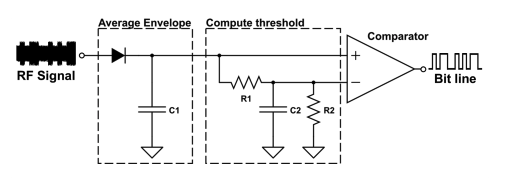
\includegraphics[scale=0.5]{backscatter_circuit}
        \label{fig:backscatter}
    \end{figure}

    Cụ thể ở bộ giải mã trong Hình 2.4, tín hiệu tán xạ ngược đầu tiên được làm mịn bởi mạch ''Average Envelope''. Sau đó mạch ''Compute threshold'' xuất ra điện áp thấp và cao của tín
    hiệu được làm mịn. Sau đó bộ so sánh ''Comparator'' so sánh tín hiệu với các ngưỡng được xác định trước để lấy ra các bit 0, 1 một cách chính xác.

\end{enumerate}

% \section{Thu hoạch năng lượng.}


\section{Học tăng cường.}
\subsection{Giới thiệu.}
Học tăng cường là quá trình học xem nên làm gì, là quá trình học để kết nối giữa trạng thái và hành động nhằm mục đích tối đa hoá một giá trị phần thưởng số học. Đối tượng học sẽ không được chỉ cụ thể là
nên thực hiện hành động nào, thay vào đó phải tự mình khám phá những hành động nào mạng lại phần thưởng cao nhất bằng cách thử chúng. Hành động của đối tượng không chỉ mang lại phần thưởng ngay lập tức mà còn ảnh hưởng
đến những trạng thái tiếp theo, dẫn đến những phần thưởng tiếp theo. Hai đặc tính thử-sai và những giá trị phần thưởng đến sau là hai đặc điểm nổi bật nhất của học tăng cường.

Học tăng cường là một nhánh của học máy, tuy nhiên nó khác biệt so với học có giám sát - là nhánh học máy được nghiên cứu nhiều nhất. Học có giám sát học từ một tập dữ liệu đào tạo đã được gán nhãn
bởi một người giám sát có kiến thức. Mỗi dữ liệu trong tập đào tạo bao gồm mô tả về tình huống và một nhãn chỉ ra hành động đúng mà hệ thống cần thực hiện trong tình huống đó. Mục tiêu là hệ thống
có thể tổng quát từ các ví dụ huấn luyện và đưa ra được dự đoán chính xác trong các tình huống mới không có trong tập dữ liệu đào tạo. Tuy nhiên học có giám sát lại không phù hợp với bài toán tương
tác, do môi trường đôi khi không rõ ràng, có nhiều yếu tố không đoán trước khiến việc thu thập dữ liệu về hành vi mong muốn là rất khó khăn, không thể thu thập đủ dữ liệu đại diện cho tất cả tình huống
mà tác nhân phải hành động. Học tăng cường cũng khác so với học không giám sát - là loại hình học tập giúp tìm ra cấu trúc ẩn trong cái tập dữ liệu chưa gán nhãn. Học tăng cường không thể được coi là
một dạng của học không giám sát dù nó cũng không dựa vào những dữ liệu có trước về hành vi đúng đắn, tuy nhiên học tăng cường có mục tiêu là tối đa giá trị phần thưởng, thay vì tìm ra cấu trúc ẩn.

Trong học tăng cường, một vấn đề cần giải quyết là yếu tố đánh đổi giữa khám phá và khai thác. Để tác nhân có thể lấy được nhiều phần thưởng, cách tốt nhất là nó sẽ ưu tiên những hành động đã thử trong
quá khứ và giành được nhiều giá trị phần thưởng. Tuy nhiên, để tìm được những hành động này, tác nhân cần thử những hành động mà nó chưa từng chọn trước đây. tác nhân cần khai thác những hành động tốt trong
quá khứ, nhưng cũng cần khám phá các hành động mới để tìm được những hành động tốt hơn trong tương lai.

\subsection{Quá trình ra quyết định Markov - MDP.}
MDP là mô hình toán học dùng để mô tả môi trường cho bài toán học tăng cường. MDP là dạng hình thức cổ điển của việc ra quyết định theo chuỗi, hành động đưa ra không chỉ ảnh hưởng đến giá trị phần thưởng
tức thì mà còn quan tâm đến những tình huống, trạng thái tiếp theo, và những phần thưởng trong tương lai. Đối tượng ra quyết định là tác nhân, thứ mà nó tương tác là môi trường. Khi tác nhân thực hiện một
hành động, môi trường phản ứng với hành động đó, thay đổi trạng thái và trả lại một số đại diện cho giá trị phần thưởng, thứ mà tác nhân sẽ tìm cách tối đa hoá theo thời gian thông qua cách nó lựa chọn các
hành động.
\begin{figure}{Tương tác giữa tác nhân và môi trường.}
    \centering
    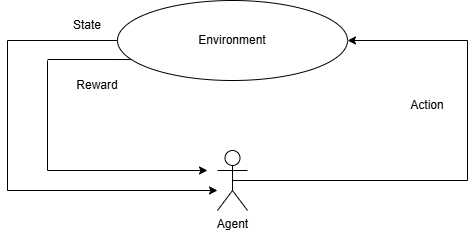
\includegraphics[scale=0.5]{mdp}
    \label{fig:mdp}
\end{figure}

Một tính chất quan trọng của MDP là: "Tương lai độc lập với quá khứ khi biết hiện tại". Khi trạng thái hiện tại được xác định, những thông tin thu được trong quá khứ sẽ không còn quan trọng để
dự đoán hành động tiếp theo. Tương lai chỉ phụ thuộc vào hiện tại chứ không phụ thuộc vào cách hệ thống đạt được trạng thái hiện tại trong quá khứ.
Về mặt toán học, một trạng thái $S_t$ có tính chất Markov khi và chỉ khi:
\[
P(s_{t+1} | s_t) = P(s_{t+1} | s_t, s_{t-1},\dots, s_1)
\]

MDP mô hình hoá một môi trường trong đó tất cả trạng thái có tính chất Markov. MDP được mô hình hoá gồm một bộ $(\mathcal{S}, \mathcal{A}, P, \mathcal{r}, \gamma)$ trong đó:
\begin{itemize}
    \item $\mathcal{S}$ là không gian trạng thái: bao gồm tất cả trạng thái của hệ thống.
    \item $\mathcal{A}$ là không gian hành động: bao gồm tất cả hành động của tác nhân.
    \item $P$ là hàm xác suất chuyển đổi trạng thái $P := \mathcal{S} \times \mathcal{A} \to [0, 1] $, biểu thị xác suất mà hệ thống chuyển từ trạng thái này đến trạng thái tiếp theo khi thực hiện
    một hành động cụ thể.
    \item $r$ là hàm giá trị phần thưởng $r := \mathcal{S} \times \mathcal{A} \times \mathcal{S} \to \mathbb{R}$, giúp xác định giá trị phần thưởng mà tác nhân nhận được khi thực hiện một hành động
    trong một trạng thái cụ thể.
    \item $\gamma \in [0, 1]$ là hệ số chiết khấu, nó đại diện cho sự đánh đổi giữa giá trị phần thưởng tức thời và những giá trị phần thưởng đến sau trong tương lai.
\end{itemize}

Dựa vào mô hình cụ thể ở trên, ta diễn tả quá trình ra quyết định Markov một cách chính thức như sau: tác nhân và môi trường tương tác với nhau theo một chuỗi các bước thời gian rời rạc
$t = 0, 1, 2,\dots$ Ở mỗi thời điểm t, tác nhân nhận được trạng thái của môi trường $s \in S$, dựa vào trạng thái này để đưa ra hành động $a \in A$. Một bước thời gian sau ở thời điểm $t+1$,
tác nhân nhận được một giá trị phần thưởng số học $r_\text{t+1} \in R$ và môi trường chuyển sang trạng thái mới $s_\text{t+1}$. Hàm xác suất chuyển đổi trạng thái $P$ thể hiện tính động của
môi trường trong MDP.

Học tăng cường là một cách giải quyết cho bài toán MDP trong trường hợp các tham số của mô hình MDP chưa xác định.

\subsection{Hàm giá trị trả về.}
Hàm giá trị trả về $R_t$ là tổng số phần thưởng tích luỹ được chiết khấu từ mốc thời gian t.
\[
R_t = r_\text{t+1} + \gamma r_\text{t+2} + \dots = \sum_{k=0}^{T} \gamma^k r_\text{t+k+1}
\]

Trong đó T là bước thời gian cuối cùng. T có thể có giá trị hữu hạn hoặc $T = \infty$. Trong trường hợp T có giá trị hữu hạn, chuỗi các tương tác giữa tác nhân và môi trường được chia thành các chuỗi
con gọi là các tập, mỗi tập kết thúc với một trạng thái được gọi là trạng thái kết thúc, sau đó môi trường sẽ được đặt lại để chuẩn bị cho một tập tiếp theo. Lấy ví dụ khi chơi một trò chơi, trạng thái
kết thúc sẽ là trạng thái thắng, thua\dots, tác nhân sẽ nhận được phần thưởng tuỳ thuộc vào trạng thái kết thúc. Các tập hoàn toàn độc lập và không ảnh hưởng đến nhau. Thời gian T cho mỗi tập có thể khác
nhau trong các tập khác nhau. Đối với trường hợp $T = \infty$, quá trình tương tác giữa tác nhân và môi trường là một quá trình liên tục và vô hạn, không có trạng thái kết thúc.

Hệ số chiết khấu $\gamma \in [0, 1]$, đại diện cho sự đánh đổi giữa giá trị phần thưởng tức thời và phần thưởng trong tương lai. Giá trị phần thưởng trong tương lai ở thời điểm k chỉ bằng $\gamma^\text{k-1}$
so với giá trị phần thưởng tức thời mà tác nhân nhận được.
\begin{itemize}
    \item Nếu $\gamma$ gần với giá trị 0, tác nhân sẽ bị coi là thiển cận, do nó chỉ quan tâm đến việc tối đa hoá giá trị phần thưởng tức thời. Điều này khiến tác nhân bỏ qua hành động có thể mang lại lợi ích 
    cao hơn về mặt lâu dài.
    \item Nếu $\gamma$ gần với giá trị 1, tác nhân sẽ được coi là nhìn xa trông rộng hơn do nó có tính đến những phần thưởng ở trong tương lai xa hơn.
\end{itemize}

Nếu MDP là quá trình theo tập (có trạng thái kết thúc) thì $\gamma$ có thể có giá trị bằng 1, tuy nhiên nếu MDP là quá trình vô hạn $(T = \infty)$ thì $\gamma$ phải có giá trị nhỏ hơn 1, để tránh trường
hợp kết quả của hàm giá trị trả về $R_t$ là một giá trị vô hạn.

\subsection{Hàm giá trị và chính sách.}
Hành động của tác nhân được xác định bởi một chính sách, kí hiệu là $\pi$, quy định cách mà tác nhân đưa ra hành động ở một trạng thái nhất định. Có hai loại chính sách là xác định và ngẫu nhiên. Chính sách xác định được
đại diện bởi hàm $\pi(s_t) = a_t$ ($a_t \in \mathcal{A}, s_t \in \mathcal{S}$) là hàm kết nối giữa một trạng thái từ không gian $\mathcal{S}$ đến một hành động từ không gian $\mathcal{A}$. Chính sách
ngẫu nhiên là một phân phối xác suất của không gian hành động $\mathcal{A}$, dựa trên trạng thái $s_t$ hiện tại: $(\pi(a_t | s_t) \in [0, 1])$. Thông qua học tăng cường, chính sách sẽ được điều chỉnh
dựa trên kinh nghiệm mà tác nhân học được.

Hàm giá trị là hàm ước tính mức độ tốt hay xấu của một tác nhân khi ở một trạng thái cụ thể dựa trên giá trị phần thưởng kì vọng. Hàm giá trị thường được xác định cùng với một chính sách $\pi$ cụ thể vì giá trị phần
thưởng trong tương lai phụ thuộc vào chuỗi hành động mà tác nhân sẽ thực hiện dưới chính sách đó.
\[
V_\pi (s) = \mathbb{E}_\pi \{R_t | s_t = s\} = \mathbb{E}_\pi \{\sum_{k=0}^{T} \gamma^k r_\text{t+k+1} | s_t = s\}, \forall s \in \mathcal{S}
\]

Trong đó kí hiệu $\mathbb{E}_\pi$ là giá trị kì vọng của biến ngẫu nhiên trong trường hợp tác nhân tuân theo chính sách $\pi$. Chúng ta gọi $V_\pi$ là hàm giá trị trạng thái cho chính sách $\pi$.

Tương tự, chúng ta cũng định nghĩa giá trị của việc lựa chọn hành động $a \in \mathcal{A}$ khi tác nhân ở trạng thái $s \in \mathcal{S}$ tuân theo chính sách $\pi$, kí hiệu là $Q_\pi (s, a)$:
\[
Q_\pi (s, a) = \mathbb{E}_\pi [R_t | s_t = s, a_t = a] = \mathbb{E}_\pi [\sum_{k=0}^{T} \gamma^k R_\text{t+k+1} | s_t = s, a_t = a]
\]

Chúng ta gọi $Q_\pi (s, a)$ là hàm giá trị trạng thái - hành động cho chính sách $\pi$, thể hiện giá trị khi tác nhân ở trạng thái s, lựa chọn hành động a.

Ta có thể biểu thị hàm giá trị trạng thái $V_\pi (s)$ như là tổng của các giá trị trạng thái - hành động của tất cả các hành động mà tác nhân có thể thực hiện ở trạng thái hiện tại, dựa trên xác suất
mà hành động đó được lựa chọn $\pi(s, a)$:
\[
V_\pi (s, a) = \sum_{a \in \mathcal{A}} \pi(s, a) Q_\pi (s, a)
\]

\subsection{Phương trình Bellman.}
Ta có thể viết lại $V_\pi(s)$ như sau:
\begin{align*}
    V_\pi(s) &= \mathbb{E}_\pi [R_t | s_t = s] \\
    &= \mathbb{E}_\pi [r_\text{t+1} + \gamma r_\text{t+2} + \dots | s_t = s] \\
    &= \mathbb{E}_\pi [r_\text{t+1} + \gamma R_\text{t+1} | s_t = s] \\
    &= \sum_{a \in \mathcal{A}} \pi (s, a) \sum_{s' \in \mathcal{S}} P(s' | s, a) [r(s, a, s') + \gamma \mathbb{E}_\pi [R_\text{t+1} | s_\text{t+1} = s']] \\
    &= \sum_{a \in \mathcal{A}} \pi (s, a) \sum_{s' \in \mathcal{S}} P(s' | s, a) [r(s, a, s') + \gamma V_\pi (s')], \forall s \in \mathcal{S}
\end{align*}
Phương trình trên mô tả mối quan hệ giữa giá trị của hàm giá trị ở trạng thái s và giá trị của hàm giá trị ở trạng thái s' là trạng thái kế tiếp của trạng thái s. Được gọi là phương trình Bellman
của $V_\pi$.

Tương tự ta cũng có phương trình Bellman cho $Q_\pi(s, a)$ như sau:
\[
Q_\pi(s, a) = \sum_{s' \in \mathcal{S}} P(s' | s, a) [r(s, a, s') + \gamma \sum_{a' \in \mathcal{A}} \pi(s', a') Q_\pi(s', a')]
\]

\subsection{Chính sách tối ưu và hàm giá trị tối ưu.}
Giải quyết bài toán MDP, hay học tăng cường có nghĩa là tìm ra một chính sách giúp tác nhân đạt được nhiều phần thưởng về lâu dài. Một chính sách $\pi$ được coi là tốt hơn một chính sách $\pi'$ nếu giá
trị trả về kì vọng $V_\pi(s)$ có giá trị lớn hơn giá trị $V_\pi'(s)$ với mọi trạng thái s. Một vấn đề có thể có một hoặc nhiều chính sách tối ưu.
\[
\pi > \pi' \iff V_\pi(s) > V_\pi'(s), \forall s \in \mathcal{S}
\]

Về mặt lý thuyết, chứng minh được rằng tồn tại một chính sách mà tốt hơn các chính sách còn lại, gọi là chính sách tối ưu (kí hiệu là $\pi^\star$). Chúng ta tìm được chính sách tối ưu $\pi^\star$ bằng
cách tìm ra hàm giá trị tối ưu $V^\star(s)$ và hàm giá trị hành động - trạng thái tối ưu $Q^\star (s, a)$:
\[
V^\star (s) = \underset{\pi}{\text{max }} V_\pi(s)
\]

Các chính sách tối ưu có cùng một hàm giá trị hành động tối ưu, kí hiệu là $Q^\star$:

\[
Q^\star (s, a) = \underset{\pi}{\text{max }} Q_\pi(s, a), \forall s \in \mathcal{S}, a \in \mathcal{A}
\]

Hàm giá trị hành động tối ưu được mô tả là giá trị phần thưởng kì vọng tối đa mà một tác nhân có thể nhận được khi thực hiện một hành động tại một trạng thái, và sau đó theo chính sách tối ưu. Do đó ta có
thể viết lại hàm $Q^\star$ dựa trên hàm $V^\star$ như sau:
\[
Q^\star (s, a) = \mathbb{E} [r_\text{t+1} + \gamma V^\star (s') | s_t = s, a_t = a]
\]

Ngoài ra mối quan hệ giữa $V^\star (s)$ và $Q^\star (s)$ còn có thể được biểu diễn như sau:
\[
V^\star (s) = \underset{a \in \mathcal{A}}{\text{max }} Q^\star (s, a)
\]

thể hiện rằng giá trị trả về tối ưu $V^\star (s)$ ở trạng thái s đạt được bằng cách chọn hành động có giá trị hành động tối ưu cao nhất.

Phương trình Bellman cho hàm giá trị tối ưu:
\begin{align*}
    V^\star (s) &= \underset{a}{max } \mathbb{E} [r(s, a, s') + \gamma V^\star (s') | s_t = s, a_t = a] \\
    &= \underset{a}{max } \sum_{s' \in \mathcal{S}} P(s' | s, a) [r(s, a, s') + \gamma V^\star (s')]
\end{align*}

\begin{align*}
    Q^\star (s, a) &= \mathbb{E} [r(s, a, s') + \gamma \underset{a'}{ max } Q^\star (s', a') | s_t = s, a_t = a] \\
    &= \sum_{s'} P(s' | s, a) [r(s, a, s') + \gamma \underset{a'}{max } Q^\star (s', a')]
\end{align*}

\section{Một số phương pháp giải quyết bài toán MDP.}
Trong phần này, chúng ta cùng xem qua một vài phương pháp có thể được sử dụng để giải quyết vấn đề MDP.

\subsection{Lập trình động - Dynamic programming.}
Lập trình động là lớp các phương thức để tìm ra những giải pháp cho bài toán MDP trong đó thông tin về tính động của môi trường là giá trị hàm $P(.|s, a)$ được biết trước. Lập trình động tìm ra
giá trị của các hàm giá trị ở các trạng thái khác nhau, qua đó tìm ra chính sách tốt.

\begin{itemize}
    \item[\textbf{a.}] \textbf{Đánh giá chính sách.}
    
    Để đánh giá một chính sách, chúng ta cần tìm ra kết quả hàm giá trị $V_\pi$ của chính sách đó. Nghĩa là chúng ta sẽ tính giá trị của hàm giá trị trạng thái $V_\pi$ của một chính sách bất kì.
    Nhắc lại phương trình Bellman đối với hàm giá trị:
    \begin{align*}
        V_\pi (s) &= \mathbb{E} [R_t | s_t = s] \\
        &= \mathbb{E} [r_\text{t+1} + \gamma R_\text{t+1} | s_t = s] \\
        &= \mathbb{E} [r_\text{t+1} + \gamma V_\pi (s_\text{t+1}) | s_t = s] \\
        &= \sum_{a} \pi(s, a) \sum_{s'} P(s' | s, a) [r(s, a, s') + \gamma V_\pi (s')]
    \end{align*}
    Để tính giá trị của $V_\pi$, chúng ta khởi tạo một giá trị $V_0$ bất kì ở trạng thái bắt đầu (nếu trạng thái được chọn là trạng thái kết thúc thì khởi tạo $V_0 = 0$), sau đó ta tính hàm giá trị
    ở trạng thái tiếp theo sử dụng công thức cập nhật sau:
    \[
    V_\text{k+1} (s) = \sum_{a} \pi (s, a) \sum_{s' | s, a} [r(s, a, s') + \gamma V_k (s')]
    \]
    Khi $k \to \infty$, chuỗi $V_k$ hội tụ đến giá trị $V_\pi$ với điều kiện $\gamma < 1$ hoặc tồn tại trạng thái kết thúc dù cho bắt đầu ở bất kì trạng thái nào. Thuật toán này gọi là thuật toán đánh giá
    chính sách.

    \item[\textbf{b.}] \textbf{Cải thiện chính sách.}
    
    Mục đích của việc tính toán hàm giá trị-trạng thái cho một chính sách bất kì ở trên là nhằm tìm ra chính sách tốt hơn. Định nghĩa chính sách $\pi'$ tốt hơn chính sách $\pi$ nếu:
    \[
    V_\pi' (s) \geq V_\pi (s), \forall s \in \mathcal{S}
    \]
    Ở trạng thái s, thay vì chọn hành động tiếp theo dựa theo chính sách $\pi$ đã xác định từ trước, ta lựa chọn một hành động khác với hành động $a = \pi(s)$ của chính sách $\pi$, sau
    đó tiếp tục tuân theo chính sách $\pi$. Như vậy ta có chính sách mới $\pi'$. Chứng minh được rằng nếu:
    \[
    Q_\pi(s, \pi'(s)) \geq V_\pi (S) \iff V_\pi' (s) \geq V_\pi (s), \forall s \in \mathcal{S}
    \]
    Có nghĩa là nếu ở trạng thái s, ta lựa chọn được hành động mới $\pi'(s)$ tốt hơn hành động của chính sách cũ $\pi(s)$, sau đó tiếp tục tuân theo chính sách $\pi$, thì chính sách mới
    $\pi'$ tốt hơn chính sách $\pi$.

    Do đó ta sẽ có phương pháp cải thiện chính sách như sau: ở mỗi trạng thái s, ta tính toán giá trị của các hành động và chọn hành động có giá trị lớn nhất, ta thu được chính sách mới
    $\pi'$ gọi là chính sách tham lam:
    \begin{align*}
        \pi' (s) &= \arg \max_{a} Q_\pi (s, a) \\
        &= \arg \max_{a} \mathbb{E} [r_\text{t+1} + \gamma V_\pi (s_\text{t+1}) | s_t = s, a_t = a] \\
        &= \arg \max_{a} \sum_{s'} P(s' | s, a) [r(s, a, s') + \gamma V_\pi(s')]
    \end{align*}

    Với $\arg \max_{a}$ là kí hiệu thể hiện việc lựa chọn hành động a để giá trị biểu thức đó lớn nhất.

    \item[\textbf{c.}] \textbf{Phương pháp lặp chính sách.}
    
    Phương pháp này phép lặp đi lặp lại một quá trình kết hợp giữa đánh gía chính sách và cải thiện chính sách, ta có một phương pháp gọi là lặp chính sách. Lựa chọn một chính sách $\pi$, chúng ta thực hiện đánh gía chính sách để tính được
    giá trị $V_\pi$, sau đó sử dụng phương pháp cải thiện chính sách để cải thiện chính sách $\pi$ để tìm ra chính sách mới $\pi'$ tốt hơn chính sách cũ. Quá trình này được lặp đi lặp lại giúp ta tìm ra chính sách tối ưu.

    \item[\textbf{d.}] \textbf{Phương pháp lặp giá trị.}
    
    Là thuật toán tìm ra chính sách tối ưu $\pi^\star$ bằng cách lặp hàm giá trị - trạng thái để tìm ra $V^\star (s)$ dựa trên phuơng trình Bellman của hàm giá trị tối ưu $V^\star$ như đã trình bày
    ở phần trước:
    \[
    V^\star (s) = \underset{a}{max } \sum_{s' \in \mathcal{S}} P(s' | s, a) [r(s, a, s') + \gamma V^\star (s')]
    \]
    Hàm giá trị tối ưu $V*$ được thực hiện bằng cách lặp với luật cập nhật hàm giá trị sau mỗi lần lặp như sau:
    \[
    V_\text{k+1} (s) = \underset{a}{max } \sum_{s'} P(s' | s, a) [r + \gamma V_k (s')]
    \]
    Quá trình lặp được thực hiện cho đến khi hội tụ (khi kết quả hàm giá trị không thay đổi quá một ngưỡng $\epsilon$ xác định trước), lúc này ta thu được hàm gía trị
    tối ưu. Chính sách tối ưu được rút ra từ hàm giá trị tối ưu như sau:
    \[
    \pi (s) = \arg \max_a \sum_{s'} P(s'|s, a) [r + \gamma V^\star (s')]
    \]
    $\pi \approx \pi^\star$ chính là chính sách tối ưu cần tìm.
    
\end{itemize}

\subsection{Phương pháp lấy mẫu Monte Carlo.}
Trong phương pháp quy hoạch động như trình bày ở trên, giả thiết cần phải biết đầy đủ về tính động của môi trường (hàm P(.|s, a) xác định), điều này đôi khi khó đạt được
trong các bài toán thực tế. Phương pháp Monte Carlo dựa trên ý tưởng không cần tính toán hàm giá trị - trạng thái $V(s)$ và hàm giá trị trạng thái - hành động
$Q(s,a)$ sử dụng hàm xác suất chuyển đổi trạng thái $P(.|s, a)$ như quy hoạch động, thay vào đó ước tính giá trị hàm $V(s)$ và $Q(s,a)$ thông qua việc lấy mẫu
một tập các hành động chuyển trạng thái của môi trường. Phương pháp Monte Carlo được trình bày như sau:
\begin{itemize}
    \item Bắt đầu từ trạng thái $s_0$.
    \item Lấy mẫu một quỹ đạo từ thời điểm t: $\tau = (s_0, a_0, r_1, s_1, a_1, \dots, s_T, a_T, r_\text{T+1}, s_\text{T+1})$ dựa trên môi trường sử dụng chính
    sách $\pi$ hiện tại.
    \item Tính toán giá trị phần thưởng tích luỹ $R_t^\text{(e)} = \sum_{k=0}^{T} \gamma^k r_\text{t+k+1}$ ở thời điểm t dựa trên quỹ đạo $\tau$
    \item Lặp lại những bước trên M lần để ước tính giá trị $V^\pi$ như sau:
    \[
    V^\pi (s) = \mathbb{E} [R_t | s_t = s] \approx \frac{1}{M} \sum_{t=1}^{M} R_t^\text{(e)}
    \]
\end{itemize}

Bằng cách lấy mẫu nhiều quỹ đạo $\tau$ từ môi trường, giá trị $V^\pi (s)$ được lấy xấp xỉ bằng cách lấy trung bình như trên. Tuy nhiên trong thực tế, khó xác
định được số mẫu quỹ đạo cần lấy để có thể ước tính giá trị được chính xác nhất. Do đó, trong thực hành, ta sẽ tiến hành cập nhật liên tục các giá trị ước tính
\[
V^\pi (s) \leftarrow V^\pi (s) + \alpha (R_t - V^\pi (s))
\]
\[
Q^\pi (s, a) \leftarrow Q^\pi (s, a) + \alpha (R_t - Q^\pi (s, a))
\]
Trong đó $\alpha \in [0, 1]$ là trọng số.

Phương pháp lấy mẫu Monte Carlo chỉ phù hợp với những bài toán mà nhiệm vụ được chia theo tập (tức là quỹ đạo theo chính sách $\pi$ hữu hạn), do nó có thể tính
được giá trị $R_t$ trong trường hợp hữu hạn, với bài toán tương tác vô hạn lần, khó để có thể lấy trung bình của phần thưởng tích luỹ.

\section{Giải quyết MDP bằng học tăng cường.}
\subsection{Học tăng cường không mô hình - Model-free RL.}
Trong học tăng cường, học tăng cường không mô hình là lớp các thuật toán học tăng cường không yêu cầu mô hình môi trường. Điều này có nghĩa là thuật toán học
không cố gắng xây dựng hoặc sử dụng một mô hình để dự đoán sự chuyển tiếp trạng thái (hàm xác suất chuyển đổi trạng thái P) hay hàm phần thưởng r. Thay vào đó, nó học thông
qua trải nghiệm từ việc tương tác trực tiếp với môi trường.

\subsection{Thuật toán học khác biệt thời gian - Temporal Difference.}
Trong phương pháp Monte Carlo, hàm giá trị $V^\pi$ được ước tính dựa vào việc tính trung bình giá trị phần thưởng tích luỹ trong mỗi tập. Tuy nhiên phương pháp Monte Carlo chỉ cập nhật
hàm giá trị sau mỗi tập, điều này dẫn đến nó không phù hợp với những vấn đề vô hạn. Phương pháp học khác biệt thời gian TD là sự kết hợp giữa ý tưởng từ phương pháp Monte Carlo và
phương pháp quy hoạch động (dynamic programming). Giống như Monte Carlo, phương pháp học TD có thể học trực tiếp từ kinh nghiệm tương tác với môi trường mà không cần nắm được tính
động của môi trường. Giống quy hoạch động ở chỗ, phương pháp TD cũng cập nhật các ước tính dựa trên những giá trị ước tính khác, mà không cần đợi đến khi kết thúc một tập mới cập
nhật giá trị như phương pháp Monte Carlo, thay vào đó phương pháp TD cập nhật giá trị ước tính ngay ở bước thời gian tiếp theo.

Phương pháp TD đơn giản nhất thực hiện cập nhật hàm giá trị như sau:
\[
V^\pi (s) \leftarrow V^\pi (s) + \alpha [\underbrace{r(s, a, s') + \gamma V^\pi (s') - V^\pi (s)}_\delta]
\]

Quá trình này có thể được mô tả như sau: ở thời điểm t, tác nhân thực hiện hành động a theo chính sách hiện tại $\pi$, quan sát giá trị phần thưởng tức thời và hệ thống chuyển sang
sang trạng thái mới s', lúc này hàm giá trị $V^\pi$ được cập nhật theo quy tắc cập nhật như trên. Trong đó $r(s, a, s') + \gamma V^\pi (s')$ là ước tính giá trị hàm $V^\pi (s)$ dựa
trên ước tính hàm giá trị của trạng thái s' tiếp theo sau khi tác nhân thực hiện hành động a và nhận phần thưởng, biểu thức $\delta = r(s, a, s') + \gamma V^\pi (s') - V^\pi (s)$ gọi là "lỗi khác biệt thời gian", 
thể hiện sự sai lệch giữa giá trị ước tính hiện tại của $V^\pi$ so với giá trị ước tính cập nhật sau khi tác nhân thực hiện hành động và nhận phần thưởng. $\alpha$ biểu thị cho tốc
độ học của tác nhân, tức là tốc độ điều chỉnh giá trị của hàm $V^\pi$ sau mỗi hành động được thực hiện. Hàm giá trị được cập nhật liên tục theo từng bước thời gian chứ không cần đợi
hết một tập (tác nhân đến trạng thái kết thúc) và không chỉ khả dụng với bài toán tương tác theo từng tập như phương pháp Monte Carlo.

Tương tự với hàm giá trị hành động $Q(s, a)$ cũng áp dụng quy tắc cập nhật tương tự trong phương pháp TD:
\[
Q^\pi (s, a) \leftarrow Q^\pi (s, a) + \alpha [\underbrace{r(s, a, s') + \gamma Q^\pi (s', a') - Q^\pi (s, a)}_\delta]
\]

Việc cập nhật giá trị hàm Q như ở trên gọi là quá trình học giá trị hàm Q, chúng ta có hai cách để tác nhân lựa chọn hành động tiếp theo khi học, cách thứ nhất, tác nhân sẽ lựa chọn
hành động dựa trên chính sách $\pi (s)$ hiện tại hoặc tác nhân lựa chọn theo hướng tham lam bằng cách chọn hành động tiếp theo $a = \arg \max_{a} Q(s', a)$. Cách lựa chọn hành động
tiếp theo của tác nhân trong phương pháp TD dẫn đến hai phương pháp:
\begin{itemize}
    \item Phương pháp theo chính sách (on-policy method): ví dụ SARSA - là một phương pháp học TD mà hành động tiếp theo của tác nhân được lựa chọn theo chính sách hiện tại $\pi (s)$.
    Chính sách nên áp dụng thêm một số phương pháp chọn hành động ví dụ như $\epsilon$ tham lam để đảm bảo khám phá được các hành động khác.

    Giá trị "lỗi khác biệt thời gian" $\delta$ được biểu diễn như sau:
    \[
    \delta = r(s, a, s') + \gamma Q^\pi (s', \pi(s')) - Q^\pi (s, a)
    \]

    \item Phương pháp không theo chính sách (off-policy method): ví dụ thuật toán Q-learning - thuật toán lựa chọn hành động dựa trên cơ chế tham lam, lựa chọn hành động có giá trị
    hàm giá trị hành động Q cao nhất để cập nhật:
    \[
    \delta = r(s, a, s') + \gamma \max_{a'} Q^\pi (s', a') - Q^\pi (s, a)
    \]

\end{itemize}

\section{Thuật toán Q-learning.}
Như đã trình bày ở phần trước, thuật toán Q-learning là thuật toán TD với phương pháp lựa chọn hành động tham lam không theo chính sách. Hàm giá trị hành động Q được cập nhật như sau:
\[
Q^\pi (s, a) \leftarrow Q^\pi (s, a) + \alpha [r(s, a, s') + \gamma \max_{a'} Q^\pi (s', a') - Q^\pi (s, a) ]
\]

Lựa chọn hành động a kế tiếp tuân theo chiến lược tham lam $\epsilon$ như sau:
\begin{align*}
    a =& \begin{cases}
        \arg \max Q(s, a) & \text{với xác suất } 1 - \epsilon, \\ 
        \text{ngẫu nhiên} & \text{với xác suất } \epsilon.
    \end{cases}
\end{align*}

Khi tác nhân lựa chọn hành động có hàm giá trị lớn nhất, tác nhân đang khai thác kinh nghiệm cũ, ưu tiên hành động đem lại nhiều phần thưởng đã được học trong quá khứ.
Khi tác nhân lựa chọn hành động ngẫu nhiên, nó đang khám phá những hành động mới nhằm tìm ra những hành động có giá trị phần thưởng cao hơn. Vấn đề cân bằng giữa khám phá và khai thác là
vấn đề quan trọng, ở thời điểm bắt đầu học, tác nhân nên ưu tiên việc khám phá thông qua lựa chọn ngẫu nhiên những hành động, càng về sau, tác nhân càng giảm tỉ lệ chọn ngẫu nhiên hành
động xuống và ưu tiên khai thác từ kinh nghiệm trong quá khứ.

\section{Học sâu tăng cường.}

\section{Mạng sâu Q - DQN.}

% Chapter 3
\chapter{Đề xuất phương pháp giải quyết bài toán gây nhiễu từ UAV.}
Trong chương này, em đề xuất phương pháp giải quyết chống nhiễu từ UAV đối với kênh truyền gồm một máy phát và một máy thu sử dụng thuật toán học tăng cường Q-learning và DQN.


\section{Mô hình hệ thống.}
Ở đây, chúng ta xem xét một hệ thống truyền thông không dây bao gồm một máy phát, một máy thu và một UAV gây nhiễu. Máy phát được trang bị bộ đệm dữ liệu để đóng vai trò như hàng đợi dữ 
liệu trước khi truyền đến máy thu, ngoài ra máy phát còn được trang bị bộ thu năng lượng và một mạch tán xạ ngược môi trường có khả năng tán xạ sóng nhiễu để truyền gói tin. Khi bị nhiễu
tấn công, máy phát có thể thu năng lượng từ tín hiệu nhiễu để sử dụng cho mục đích truyền gói tin chủ
động đến máy thu sau này khi máy gây nhiễu không tấn công - chế độ HTT, hoặc tán xạ ngược dữ liệu dựa trên sóng nhiễu - chế độ tán xạ ngược.

\begin{figure}{Mô hình hệ thống.}
    \centering
    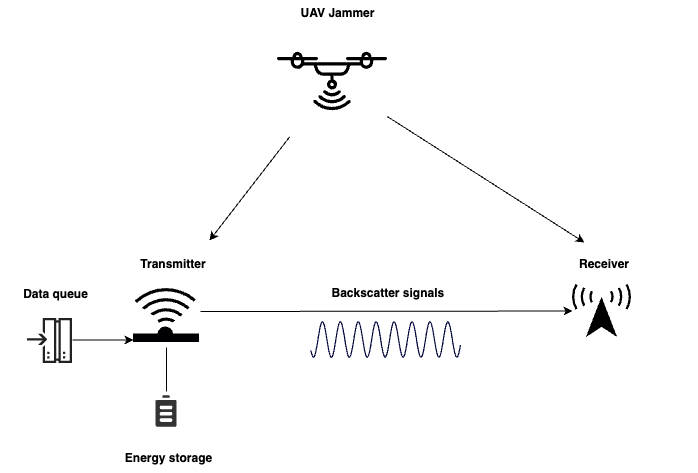
\includegraphics[scale=0.5]{system_model}
    \label{fig:system_model}
\end{figure}

\subsection{Mô hình gây nhiễu.}
Chúng ta xem xét một UAV có khả năng gây nhiễu thông minh. Giả sử UAV có khả năng lắng nghe kênh truyền giữa máy phát và máy thu khi tấn công. Điều này cho phép UAV có thể điều chỉnh vị trí
cũng như chiến lược gây nhiễu để tối đa hoá thiệt hại lên kênh truyền giữa máy phát và máy thu. Mục tiêu của UAV là làm giảm giá trị SINR tại máy thu, khiến cho kênh thông lượng của kênh
truyền giảm xuống, giá trị SINR được tính như đã trình bày ở phần cơ sở lý thuyết như sau:
\[
\theta = \frac{P_R}{\varphi P_J + \rho^2}
\]
Trong đó $P_R$ là công suất nhận được từ máy phát tại cổng (máy thu), $P_J$ là công suất nhiễu được phát của máy gây nhiễu, $\rho^2$ là phương sai của nhiễu Gauss trắng cộng thêm. 
$\varphi P_J$ là công suất nhiễu tại cổng, trong đó $0 \leq \varphi \leq 1$ là hệ số suy giảm kênh truyền.

Giá trị công suất sóng nhiễu $P_J$ của UAV tác động lên máy thu là giá trị thay đổi do UAV có khả năng thay đổi vị trí để tối ưu hoá khả năng tấn công kênh truyền như giả thiết ở trên.
Khi UAV đến gần máy phát và máy thu, khả năng xuất hiện đường truyền LoS tăng lên do góc nâng $\theta_i$
tăng lên, dẫn đến cường độ nhiễu tác động lên máy phát và máy thu tăng lên. Ngược lại khi UAV di chuyển ra xa máy phát và máy thu, khả năng gặp vật cản và các yếu tố như tăng khả năng kênh
truyền NLoS, dẫn đến cường độ nhiễu tác động lên máy phát và máy thu giảm. Ngoài ra, sẽ có những thời điểm sóng nhiễu từ UAV không tác động đến máy phát và máy thu, do sóng nhiễu có thể không
truyền đến được máy phát và máy thu do yếu tố vật cản từ môi trường, hoặc do UAV là thiết bị hạn chế về mặt năng lượng, nên có những thời điểm nó cần quay lại trạm để thay pin để bổ sung năng
lượng, khi đó UAV không tấn công kênh truyền hay cường độ gây nhiễu của UAV lên máy phát và máy thu là 0W.

Ta giả sử $P_J = \{P_0^J, \dots, P_n^J, \dots, P_N^J\}$ là vector tập các giá trị cường độ nhiễu khác nhau trong các thời điểm khác nhau của UAV. Tại mỗi thời điểm, do sự thay đổi vị trí
hoặc do yếu tố môi trường\dots, cường độ nhiễu từ UAV là khác nhau và là một trong những giá trị trong vector $P_J$ với giá trị xác suất là $x_n$. Trong đó giá trị nhỏ nhất trong vector $P_J$
là 0W, tương ứng với những thời điểm sóng nhiễu từ UAV không tác động đến kênh truyền như đã trình bày ở trên.

Ta kí hiệu $J_s = \{x = (x_0, \dots, x_n\dots, x_N), \sum_{i=0}^{N}x_n = 1\}$ là vector xác suất tấn công của UAV tương ứng với các mức năng lượng trong vector $P_J$, hay $J_s$ còn được coi như
là chiến lược tấn công của UAV.

Do UAV là thiết bị hạn chế về mặt năng lượng, UAV xác định một chiến lược tấn công $J_s$ sao cho mức công suất nhiễu trung bình $P_\text{avg}$ phù hợp với mức năng lượng và trạng thái hiện tại của UAV.
Do giả thiết UAV gây nhiễu thông minh có khả năng lắng nghe kênh truyền, chúng ta giả sử UAV gây nhiễu sẽ nhận về một phần thưởng $w_n^J$ tương ứng với mỗi giá trị $P_n^J$ trong vector $P_J$, đại diện
cho số gói tin từ máy phát đến máy thu không thành công do tác động từ sóng nhiễu (ví dụ do không giải mã thành công tại máy thu do SINR giảm). Kí hiệu $w_J = \{w_0^J, \dots, w_n^J, \dots, w_N^J\}$
là vector phần thưởng của UAV gây nhiễu. Mục tiêu của UAV gây nhiễu được xác định như sau:
\begin{align*}
    \begin{cases}
        \underset{x}{\max} \, x w_J^\top, \\
        \sum_{n=0}^{N} x_n = 1, x_n \in [0, 1], \forall n \in \{0, \dots, N\}, \\
        x P^T \leq P_\text{avg} \\
    \end{cases}
\end{align*}

Mục tiêu của UAV bao gồm tối đa hoá thiệt hại của đường truyền, nhưng đồng thời cũng điều chỉnh chiến lược tấn công phù hợp với trạng thái hiện tại của UAV.

\subsection{Mô hình kênh truyền.}
Khi UAV gây nhiễu không tấn công kênh truyền, hoặc khi tín hiệu nhiễu từ UAV không tác động đến kênh truyền do vật cản, máy phát có thể phát chủ động $\hat{d}_t$
gói tin đến máy thu (sử dụng phương pháp truyền dẫn chủ động thông thường), hoặc không hoạt động. Mỗi gói tin truyền thành công cần $e_t$ đơn vị năng lượng.
Khi UAV gây nhiễu tấn công và nằm trong phạm vi ảnh hưởng đến kênh truyền, máy phát vẫn có thể hoặc phát gói tin đến máy thu bằng cách điều chỉnh tốc độ phát tương
ứng với cường độ nhiễu sử dụng kỹ thuật RA, hoặc thu năng lượng từ sóng nhiễu, hoặc tán xạ ngược tín hiệu nhiễu để truyền dữ liệu đến máy thu. Thông qua các thí nghiệm
và phân tích về các hệ thống truyền thông tán xạ ngược, có thể thấy rằng với sóng nhiễu với cường độ càng lớn, càng nhiều gói tin có thể tán xạ ngược đến máy thu, và cũng
càng nhiều năng lượng có thể thu được từ sóng nhiễu nếu máy phát hoạt động ở chế độ thu năng lượng. 

Cụ thể, trong trường hợp máy
phát chọn điều chỉnh tốc độ phát dùng kĩ thuật RA, đặt $r = \{r_1, \dots, r_m,\dots, r_M\}$ là tập hợp các tốc độ truyền mà máy thu có thể lựa chọn để truyền khi bị tấn
công. Ở mỗi tốc độ $r_m$, máy phát có thể truyền tối đa $\hat{d_m^t}$ gói tin. Với $m = 1, \dots, M$ khi $\gamma_{m-1} \leq \theta < \gamma_m$ với $\gamma_m$ là giá
trị của SINR, máy thu chỉ có thể giải mã những gói tin được gửi ở tốc độ $r_0, r_1, \dots, r_\text{m-1}$, những gói tin gửi ở tốc độ $r_m$ hoặc cao hơn sẽ bị mất,
do máy thu không giải mã được. 

Trong trường hợp máy phát chọn thu năng lượng từ sóng nhiễu, năng lượng này có thể được sử dụng cho quá trình truyền chủ động sau này, tương ứng với mỗi mức cường độ nhiễu $P_n^J$
ảnh hưởng đến máy phát khác nhau, máy phát có thể thu được $e_n^J$ đơn vị năng lượng. Kí hiệu $e = \{e_0^J, \dots, e_N^J\}$ là các giá trị năng lượng có thể thu được tương ứng
với các mức nhiễu khác nhau của UAV.

Trong trường hợp máy phát chọn tán xạ ngược sóng nhiễu để truyền dữ liệu đến máy thu, kí hiệu $\hat{d_n^J}$ là số gói tin tối đa có thể được tán xạ ngược bởi máy phát nếu
cường độ nhiễu tương ứng là $P_n^J$. Lưu ý rằng tốc độ tán xạ ngược dữ liệu được quy định bởi mạch tán xạ ngược và không thay đổi và kí hiệu là $b^{\dagger}$. Trong mô hình đề xuất này
, chúng ta giả sử khi máy phát lựa chọn tán xạ ngược sóng nhiễu, nó có thể truyền được $b^{\dagger}$ gói tin, nếu $b^{\dagger} > \hat{d_n^J}$ thì $(b^{\dagger} - d_n^J)$ gói tin sẽ bị mất trong
quá trình tán xạ ngược dữ liệu. Kí hiệu $\hat{d} = \{\hat{d_0^J}, \dots, \hat{d_N^J}\}$ là vector thể hiện số gói tin có thể được tán xạ ngược tương ứng với cường độ nhiễu.

Chúng ta kí hiệu D và E tương ứng là kích cỡ bộ đệm dữ liệu và lượng năng lượng tối đa mà máy phát có thể lưu trữ. Quá trình gói tin đến máy phát được giả sử tuân theo phân
phối Poisson với tốc độ trung bình $\lambda$. Khi bộ đệm dữ liệu của máy phát đầy, gói tin mới đến sẽ bị loại bỏ.

Lưu ý là trong hệ thống đề xuất này, máy phát chỉ có thể xác định nó có đang bị tấn công gây nhiễu hay không mà không biết cụ thể cường độ của sóng nhiễu. Thuật toán đề xuất sử dụng học tăng 
cường sâu có khả năng học được thông tin về chiến lược tấn công của UAV, cường độ của sóng nhiễu và những khả năng liên quan, qua đó đưa ra lựa chọn
phù hợp nhằm làm tối đa thông lượng trung bình của kênh truyền.


\section{Công thức hoá vấn đề.}
Để đối phó với cuộc tấn công gây nhiễu từ UAV vốn có tính động và không chắc chắn, chúng ta xây dựng vấn đề tối ưu hoá của hệ thống được đề cập ở trên như một quá trình ra quyết định
Markov (MDP). Việc mô hình hoá này giúp máy phát có thể ra quyết định tối ưu nhằm tối đa hoá giá trị phần thưởng dài hạn, trong trường hợp này là giá trị thông lượng trung bình
của hệ thống truyền thông. MDP được xác định bởi một bộ $\langle S, A, r \rangle$ trong đó S là không gian trạng thái, A là không gian hành động và r là hàm giá trị phần thưởng
tức thời của hệ thống.

\subsection{Không gian trạng thái.}
Chúng ta xác định không gian trạng thái của hệ thống trong trường hợp này bao gồm ba trạng thái là trạng thái tấn công của máy gây nhiễu UAV, trạng thái của bộ đệm dữ liệu máy phát và trạng thái của bộ lưu
trữ năng lượng của máy phát.
\[
\mathcal{S} = \{(j, d, e) : j \in \{0, 1\}; d \in \{0, \dots, D\}; e \in \{0, \dots, E\}\}
\]

Trong đó j là trạng thái UAV gây nhiễu, với $j = 0$ nếu như UAV không tấn công hoặc $j = 1$ nếu sóng nhiễu của UAV tấn công kênh truyền, d và e tương ứng là số gói tin trong bộ
đệm và số đơn vị năng lượng trong bộ lưu trữ năng lượng của máy phát. Trạng thái của hệ thống được xác định bởi một biến tổng hợp $s = (j, d, e) \in S$.

\subsection{Không gian hành động.}
Máy phát có thể thực hiện $(M+4)$ hành động trong không gian trạng thái $\mathcal{A}$, bao gồm không hoạt động, truyền dữ liệu chủ động, thu thập năng lượng từ sóng nhiễu, tán xạ ngược sóng
nhiễu và điều chỉnh tốc độ phát là một trong M giá trị tốc độ của vector $r = \{r_1, \dots, r_m,\dots, r_M\}$ bằng cách sử dụng kĩ thuật RA khi sóng nhiễu từ UAV ảnh hưởng đến
kênh truyền (UAV tấn công). Do đó, không gian hành động được xác định là tập $]\mathcal{A} = \{a : a \in \{1, \dots, M+4\}\}$ trong đó:

\begin{align*}
    a &= \begin{cases}
        1, & \text{Không hoạt động,} \\
        2, & \text{Truyền dữ liệu chủ động,} \\
        3, & \text{Thu hoạch năng lượng từ sóng nhiễu,} \\
        4, & \text{Tán xạ ngược dữ liệu trên sóng nhiễu,} \\
        4 + m, & \text{Điều chỉnh tốc độ phát sang } \\
                & r_m \text{ với } m \in \{1, \ldots, M\}.
    \end{cases}
\end{align*}

\subsection{Phần thưởng tức thời.}
Trong mô hình này, phần thưởng tức thời sau khi thực hiện hành động a ở trạng thái s là số gói tin được truyền thành công đến máy thu. Do đó hàm giá
trị phần thưởng tức thời được biểu diễn như sau:

\begin{align*}
    r(s,a) &= \begin{cases}
        d_t, & (j = 0, d > 0, e \geq e_t, a = 2; 0 < d_t \leq \hat{d_t}) \\
        d_n^J, & (j = 1, d > 0, a = 4; 0 < d_n^J \leq \hat{d_n^J}) \\
        d_m^r, & (j = 1, d > 0, e \geq e_t, a = 4 + m; 0 < d_m^r \leq \hat{d_m^r}) \\
        0, & \text{Trong các trường hợp còn lại.} \\
    \end{cases}
\end{align*}

Khi UAV gây nhiễu không tấn công kênh truyền (j = 0), máy phát có dữ liệu trong bộ đệm và có đủ năng lượng trong bộ lưu trữ, lúc này nó có thể chọn phát
chủ động gói tin đến máy thu (a = 2), số gói tin có thể truyền đến máy thu là $d_t$ gói tin thoả mãn $0 < d_t \leq \hat{d_t}$ gói tin (trong đó $\hat{d_t}$
là số gói tin tối đa mà máy phát có thể phát chủ động).

Khi máy gây nhiễu tấn công kênh truyền (j = 1), máy phát có gói tin trong bộ đệm $(d > 0)$, nó có thể tán xạ ngược sóng nhiễu để truyền dữ liệu đến máy thu (a = 4), 
số gói tin tán xạ ngược thành công là $d_n^J$ gói tin trong đó $0 < d_n^J \leq \hat{d_n^J}$. (Trong đó $\hat{d_n^J}$ là số gói tin tối đa mà máy phát có thể tán xạ ngược
ở cường độ nhiễu là $P_n^J$).

Ngoài ra khi máy gây nhiễu tấn công (j = 1), máy phát có gói tin trong bộ đệm $(d > 0)$ và có đủ năng lượng $(e \geq e_t)$, nó còn có thể lựa chọn phát gói 
tin với tốc độ $r_m$, (a = 4 + m) để truyển chủ động gói tin theo kĩ thuật RA, số gói tin truyền thành công đến máy thu là $d_m^r$ trong đó $0 < d_m^r \leq \hat{d_m^r}$.
($\hat{d_m^r}$ là số gói tin tối đa mà máy phát có thể phát thành công nếu máy phát phát với tốc độ $r_m$).

Trong các trường hợp còn lại, khi máy phát không truyền thành công gói tin đến máy thu thì giá trị phần thưởng tức thời là 0.


\subsection{Công thức tối ưu hoá.}
Mục tiêu của chúng ta là tìm ra một chính sách tối ưu cho máy phát, được kí hiệu là $\pi^*$, nhằm làm tối đa hoá giá trị thông lượng trung bình
của hệ thống. Cụ thể $\pi^*$ là ánh xạ từ một trạng thái nhất định của hệ thống (trạng thái nhiễu, trạng thái bộ đệm dữ liệu và trạng thái năng
lượng của máy phát) đến một hành động tối ưu ở trạng thái đó.
Công thức hàm tối ưu hoá được xác định như sau:
\[
\max_{\pi} R(\pi) = \lim_{T \to \infty} \frac{1}{T} \sum_{k=1}^{T} \mathbb{E}\left( r_k(s_k, \pi(s_k)) \right)
\]

Trong đó $R(\pi)$ là giá trị thông lượng trung bình của máy phát tuân theo $\pi$.

$r_k(s_k, \pi(s_k))$ là giá trị phần thưởng tức thời ở thời điểm $k$ sau khi thực hiện hành động $a_k$ ở trạng thái $s_k$. 

$\pi(s_k) = a_k$ là hành động tại thời điểm k tuân theo chính sách $\pi$.

Do trong mô hình MDP được xây dựng cho bài toán này, các trạng thái trong không gian trạng thái $S$ thuộc cùng một lớp liên kết trong chuỗi Markov, nên chuỗi Markov này là chuỗi không thể giảm bớt.
Khiến cho với mọi chính sách $\pi$, thông lượng trung bình $R(\pi)$ là một giá trị xác định và không phụ thuộc vào trạng thái bắt đầu của chuỗi.

\section{Áp dụng phương pháp học tăng cường Q-learning và học tăng cường sâu DQN để chống nhiễu.}
Trong hệ thống được đề xuất ở trên, máy phát không xác định được cụ thể mức độ nhiễu mà UAV gây ra trên kênh truyền, cũng như chiến lược tấn công của UAV để có thể tìm ra được
chính sách tối ưu $\pi^\star$ để tối đa hoá thông lượng kênh truyền. Do đó chúng ta sẽ áp dụng các thuật toán học tăng cường để giúp máy phát tìm ra được chiến lược đối
phó với máy gây nhiễu, hay nói cách khác là lựa chọn những hành động đúng trong không gian hành động $\mathcal{A}$ để đạt được thông lượng trung bình cao nhất.

\subsection{Sử dụng thuật toán học tăng cường Q-learning.}
Thuật toán Q-learning sử dụng một bảng gọi là bảng Q nhằm lưu giữ giá trị của các cặp trạng thái và hành động tương ứng của máy phát. Dựa trên trạng thái hiện tại, máy phát đưa ra hành động dựa trên
chiến lược phòng thủ hiện tại của nó. Sau khi thực hiện hành động, máy phát quan sát phần thưởng nhận được và trạng thái tiếp theo sau đó tiến hành cập nhật bảng Q, thực hiện việc này lặp đi lặp lại nhiều lần. 
Bằng cách này, máy phát có thể học cách đưa ra quyết định đúng dựa trên kinh nghiệm của chính nó, qua đó đạt được một chiến lược phòng thủ tối ưu $\pi^\star$: là một liên kết giữa trạng thái và hành động tương
ứng mà máy phát sẽ lựa chọn để tối đa hoá thông lượng, giảm số gói tin bị mất khi bị UAV tấn công.

Kí hiệu $V^\pi (s)$ là giá trị phần thưởng kì vọng mà máy phát sẽ nhận được khi tuân theo chính sách $\pi$ ở trạng thái $s \in \mathcal{S}$:
\[
V_\pi (s) = \mathbb{E}_\pi \{\sum_{k=0}^{\infty} \gamma^k r_\text{t+k+1} | s_0 = s\} = \mathbb{E}_\pi [r + \gamma V^\pi (s_\text{t+1}) | s_0 = s]
\]
Với $0 \leq \gamma < 1$ là hệ số chiết khấu, đại diện cho sự đánh đổi giữa phần thưởng tức thời và phần thưởng trong tương lai, nếu $\gamma$ gần giá trị 0, thuật toán sẽ lựa chọn những hành động để
tối đa giá trị phần thưởng tức thời, còn nếu $\gamma$ gần với giá trị 1, máy phát sẽ lựa chọn những hành động để tối đa hoá giá trị phần thưởng tích luỹ về lâu dài, hay nói cách khác là tác nhân sẽ nhìn xa
trông rộng hơn.

Tìm ra chính sách tối ưu $\pi^\star$ là mục tiêu của thuật toán này, hàm giá trị tối ưu và hàm giá trị hành động tối ưu được định nghĩa như sau:
\[
V^\star (s) = \underset{a}{\max} \mathbb{E} [r(s, a, s') + \gamma V^\star (s')]
\]
\[
Q^\star (s, a) = \mathbb{E} [r(s, a, s') + \gamma \underset{a'}{ max } Q^\star (s', a') | s_t = s, a_t = a]
\]

Hàm giá trị tối ưu có mối quan hệ với hàm giá trị hành động tối ưu như sau:
\[
V^\star (s) = \underset{a \in \mathcal{A}}{\text{max }} Q^\star (s, a)
\]

Thuật toán Q-learning là thuật toán TD với cơ chế lựa chọn hành động tiếp theo không theo chính sách hiện tại mà lựa chọn hành động có giá trị
$Q(s, a)$ cao nhất. Bằng việc thực hiện phép lặp và cập nhật giá trị hàm $Q(s, a)$ liên tiếp, hàm $Q(s, a)$ sẽ hội tụ đến một chiến lược tối ưu $\pi^\star$.
Hàm $Q(s, a)$ được cập nhật như sau:
\[
Q_\text{t+1} (s_t, a_t) = Q_t (s_t, a_t) + \alpha_t [r_t(s_t, a_t, s_\text{t+1}) + \gamma \max_{a_\text{t+1}} Q_t (s_\text{t+1}, a_\text{t+1}) - Q_t (s_t, a_t) ]
\]

Biểu thức $\delta = r_t(s_t, a_t, s_\text{t+1}) + \gamma \max_{a_\text{t+1}} Q_t (s_\text{t+1}, a_\text{t+1}) - Q_t (s_t, a_t)$ là giá trị thể hiện sự sai khác
giữa giá trị hàm Q được dự đoán và giá trị hàm Q hiện tại. Hệ số $\alpha_t$ gọi là tốc độ học, định nghĩa tác động của giá trị mới lên giá trị hiện tại. Để đảm bảo thuật toán
Q-learning hội tụ, tìm được chính sách tối ưu, tốc độ học $\alpha_t$ thoả mãn điều kiện sau:
\[
\sum_{t=0}^{\infty} \alpha_t (s, a) = \infty, \text{và } \sum_{t=0}^{\infty} \alpha_t^2 (s, a) < \infty
\]
\begin{algorithm}
    \caption{Thuật toán chống nhiễu dựa trên lập bảng Q-learning.}\label{alg:qlearning}
    \begin{algorithmic}[1]
    \State \textbf{Initialize } $Q_0(s,a) = 0 \forall s,a.$, learning rate $\alpha$ and discount factor $\gamma$
    
    \For{t = 1 to T}
        \State From current state $s_t$, choose action $a_t$ based on $\epsilon$-greedy and and execute, obtain the immediate reward
        $r_t$ and new state $s_\text{t+1}$. Select an action $a_\text{t+1}$ based on the state $s_{t+1}$ and then update the table entry for $Q(s_t, a_t)$
        as follows:
        \[
        Q_\text{t+1} (s_t, a_t) = Q_t (s_t, a_t) + \alpha_t [r_t(s_t, a_t, s_\text{t+1}) + \gamma \max_{a_\text{t+1}} Q_t (s_\text{t+1}, a_\text{t+1}) - Q_t (s_t, a_t) ]
        \]
        \State Replace $s_t \leftarrow s_\text{t+1}$
    \EndFor
    \State \textbf{Output: } $\pi^\star (s) = \arg \max_{a} Q^\star (s, a)$
\end{algorithmic}
\end{algorithm}

Hành động a được lựa chọn theo chiến lược $\epsilon$-greedy như sau: ở lần lặp thứ k
\begin{align*}
    a =& \begin{cases}
        \arg \max Q(s, a) & \text{với xác suất } 1 - \epsilon, \\ 
        \text{ngẫu nhiên} & \text{với xác suất } \epsilon.
    \end{cases}
\end{align*}

\subsection{Phương pháp học tăng cường sâu DQN.}
Vấn đề của thuật toán Q-learning là tốc độ hội tụ thấp, đồng thời không khả thi với bài toán dữ liệu nhiều chiều. Ngoài ra với thuật toán lập bảng Q-learning,
khi có số lượng lớn các hành động và trạng thái, thuật toán gặp vấn đề bộ nhớ khi kích thước bảng Q lớn, do không gian trạng thái $\mathcal{S}$ và không gian hành động $\mathcal{A}$
lớn, số lượng cặp trạng thái - hành động $(s,a)$ cũng sẽ rất lớn, điều này dẫn đến bảng Q cần phải lưu trữ một lượng dữ liệu khổng lồ. Tốc độ cập nhật bảng Q và tốc độ hội tụ cũng sẽ
chậm hơn rất nhiều.

Ở đây em đề xuất một thuật toán tìm ra chiến lược phòng thủ tối ưu cho máy phát dựa trên học sâu sử dụng mạng thần kinh nhân tạo. Thuật toán học sâu DQN được đề xuất bởi Google Deepmind 
sử dụng mạng thần kinh sâu để ước tính giá trị xấp xỉ của hàm giá trị hành động tối ưu $Q^\star (s, a)$. Thuật toán sử dụng một số cơ chế sau:
\begin{itemize}
    \item Cơ chế lưu trữ, phát lại trải nghiệm: Thuật toán sử dụng một bộ nhớ phát lại D, là bể dữ liệu để lưu các kinh nghiệm của quá trình chuyển đổi trạng thái $(s_t, a_t, r_t, s_\text{t+1})$
    thay vì ngay lập tức đào tạo mạng thần kinh sử dụng các cặp trạng thái hành động diễn ra trong quá trình trải nghiệm. Tiến hành lấy ngẫu nhiên từ bể dữ liệu, sau đó đưa vào
    mạng thần kinh sâu để đào tạo. Cách làm này giúp thuật toán học hiệu quả những kinh nghiệm cũ nhiều lần và loại bỏ mối tương quan trong các mẫu.

    \item  Sử dụng một mạng Q mục tiêu: Trong thuật toán DQN, ta sử dụng hai mạng Q có kiến trúc giống hệt nhau, một mạng Q mục tiêu và một mạng Q chính. Việc sử dụng mạng Q 
    mục tiêu giúp cải thiện tính ổn định trong quá trình học. Cụ thể, mạng Q mục tiêu giảm thiểu sự dao động mạnh mẽ của giá trị Q bằng cách cập nhật ít thường xuyên hơn so với
    mạng Q chính. Điều này giúp giảm hiện tượng ước lượng quá mức và tránh làm mất ổn định quá trình học, nhờ đó quá trình hội tụ trở nên ổn định và nhanh chóng hơn.
\end{itemize}

\begin{algorithm}
    \caption{Thuật toán chống nhiễu sử dụng DQN.}\label{alg:dqn}
    \begin{algorithmic}[1]
    \State Initialize replay memory D
    \State Initialize the Q-network $\mathcal{Q}$ with random weights $\theta$.
    \State Initialize the target Q-network $\hat{\mathcal{Q}}$ with weight $\theta' = \theta$.
    \For{t = 1 to T}
        \State With probability $\epsilon$ select a random action $a_t$, otherwise select $a_t = \arg \max \mathcal{Q}^\star (s_t, a_t, \theta)$
        \State Perform action $a_t$ and observe reward $r_t$ and next state $s_\text{t+1}$
        \State Store transition $(s_t,a_t,r_t,s_\text{t+1})$ in the replay memory D
        \State Sample random mini-batch of transitions $(s_j,a_j,r_j,s_\text{j+1})$ from D
        \State $y_j = r_j + \gamma \max_{a\text{j+1}} \hat{\mathcal{Q}} (s_\text{j+1}, a_\text{j+1}, \theta')$
        \State Perform a gradient descent step on $(y_j - \mathcal{Q} (s_j, a_j, \theta))^2$.
        \State Every C steps reset $\hat{\mathcal{Q}} = \mathcal{Q}$
    \EndFor
\end{algorithmic}
\end{algorithm}

Trong thuật toán DQN ở trên quá trình đào tạo bao gồm T tập. Trong mỗi tập, ở trạng thái hiện tại, tác nhân lựa chọn một hành động dựa trên chiến lược tham lam $\epsilon$.
Ban đầu, hành động được lựa chọn theo một chính sách ngẫu nhiên, sau khi học được kinh nghiệm từ phần thưởng nhận được, tác nhân dần xác định một chính sách cố định mà ở
đó thu được nhiều phần thưởng nhất. Cụ thể thì ban đầu giá trị $\epsilon$ là một số gần với 1, sau đó giảm dần xuống một giá trị nhỏ dựa trên một hệ số suy giảm nhất định.
Điều này giúp tác nhân tự do khám phá những hành động tiềm năng từ lúc bắt đầu, càng về sau, khi giá trị $\epsilon$ giảm, tác nhân sẽ chọn những hành động có giá trị Q lớn
nhất, nhằm khai thác những kiến thức đã học được để tối đa hóa phần thưởng. Điều này giúp thuật toán học hỏi một cách hiệu quả, vừa đảm bảo sự ổn định trong quá trình
huấn luyện, vừa đảm bảo khả năng khai thác khám phá để tối ưu chiến lược về dài hạn.

Sau đó, tác nhân tiến hành thực hiện hành động, quan sát trạng thái kế tiếp và nhận về phần thưởng. Quá trình chuyển đổi này được lưu trong bộ nhớ phát lại D để cho
quá trình đào tạo về sau.

Trong quá trình học tập, một số mẫu được lấy ngẫu nhiên từ bộ nhớ phát lại D và được đưa vào mạng thần kinh. Thuật toán cập nhật tham số mạng bằng giảm thiểu hàm mất mát
sử dụng SGD:
\[
L_i(\theta_i) = \mathbb{E}_{(s, a, r, s') \sim U(D)} \left[ \left( r + \gamma \max_{a'} \mathcal{Q}(s', a'; \theta'_i) - \mathcal{Q}(s, a; \theta_i) \right)^2 \right]
\]
Trong đó $\theta_i$ là tham số của mạng chính Q ở tập đào tạo thứ i và $\theta_i'$ là tham số của mạng mục tiêu $\hat{\mathcal{Q}}$

Sau C bước, thuật toán cập nhật tham số mạng mục tiêu $\theta_i'$ với tham số của mạng chính $\theta_i$.

Sau khi quá trình đào tạo kết thúc, tham số từ mạng chính $\mathcal{Q}$ được sử dụng để giúp máy phát đưa ra quyết định để tối ưu hoá thông lượng.

% Chapter 4
\chapter{Thiết lập mô phỏng và đánh giá hiệu năng.}
\section{Thông số cài đặt thử nghiệm.}
\subsection{Thông số hệ thống.}
Trong hệ thống đang được xem xét, máy phát có thể lưu trữ tối đa $D = 10$ gói tin trong hàng đợi dữ liệu, tối đa $E = 10$ đơn vị năng lượng
trong bộ lưu trữ năng lượng. Dữ liệu đến máy phát giả định tuân theo phân phối Poisson với tốc độ trung bình $\lambda = 3$ 
gói tin. Khi UAV gây nhiễu không tấn công, máy phát có thể truyền chủ động tối đa $\hat{d}_t = 4$ gói tin đến máy thu. Mỗi gói tin truyền đi cần
$e_t = 1$ đơn vị năng lượng. Do sự thay đổi vị trí của UAV như đã nói ở trên, công suất gây nhiễu của UAV cũng thay đổi, giả định tín hiệu nhiễu từ 
UAV ảnh hưởng đến đường truyền không dây đang xét gồm bốn mức $P_J = \{0W, 5W, 10W, 15W\}$ với $P_{\text{max}} = 15W$. Do lượng năng lượng
thu hoạch được cũng như số gói tin tán xạ ngược thành công tăng lên khi tín hiệu nhiễu mạnh hơn, chúng ta đặt $e = \{0, 1, 2, 3\}$ là số đơn vị
năng lượng mà máy thu có thể thu được và $\hat{d} = \{0, 1, 2, 3\}$ là số gói tin mà máy thu có thể tán xạ ngược tương ứng với mức công suất nhiễu
ảnh hưởng tới đường truyền. Ngoài ra, khi UAV tấn công gây nhiễu và máy phát sử dụng kỹ thuật RA, nó có thể truyền $d^r_m = \{2, 1, 0\}$ gói tin
tương ứng với cường độ tín hiệu nhiễu từ UAV $P^J_n = \{5W, 10W, 15W\}$. Công suất nhiễu trung bình của UAV là $P_\text{avg} = 7W$.

\subsection{Thông số cài đặt thuật toán Q-learning và DQN.}
\begin{itemize}
    \item[\textbf{a.}] \textbf{Thuật toán Q-learning.}
    
    Trong mô phỏng tìm ra chiến lược tối ưu cho mô hình hệ thống ở trên sử dụng thuật toán Q-learning, ta đặt các thông số như sau: tốc độ học $\alpha = 0.1$,
    hệ số chiết khấu $\gamma = 0.9$. Ngoài ra còn áp dụng chiến lược $\epsilon$ tham lam với $\epsilon = 1$, giá trị $\epsilon$ giảm dần xuống giá trị $\epsilon_\text{min} = 0.01$,
    với tốc độ giảm giá trị $\epsilon_\text{decay} = 0.01$. Số lần lặp $T = 10^6$.
    \item[\textbf{b.}] \textbf{Thuật toán DQN.}
    
    Trong mô phỏng thuật toán DQN, kiến trúc của mạng mục tiêu $\hat{\mathcal{Q}}$ và mạng chính $\mathcal{Q}$ là như nhau: mô hình sử dụng kiến trúc DQN chuẩn, 
    gồm ba lớp ẩn với 512, 256, và 64 neuron, mỗi lớp sử dụng hàm kích hoạt tanh. Lớp đầu ra có $M+4$ neuron tương ứng với kích cỡ không gian hành động của hệ thống 
    và sử dụng hàm kích hoạt linear để xuất ra giá trị Q cho từng hành động. Giá trị ban đầu của $\epsilon$ trong chiến lược $\epsilon$ tham lam là $\epsilon = 1$,
    $\epsilon_min = 0.01$, hệ số suy giảm giá trị $\epsilon$ là $\epsilon_\text{decay} = 0.9999$. Tốc độ học (learning rate) là $\alpha = 0.0001$. Kích cỡ của bộ
    nhớ phát lại là $D = 10000$, số mẫu được lấy ngẫu nhiên ở mỗi lần đào tạo mạng từ bộ nhớ phát lại (mini-batch) là 32 mẫu, mạng mục tiêu $\hat{\mathcal{Q}}$ được cập
    nhật tham số với tần suất là 5000 bước huấn luyện.
\end{itemize}

\section{Kết quả mô phỏng.}
\subsection{So sánh sự hội tụ của hai thuật toán học tăng cường Q và DQN.}
Trong Hình 4.1, chúng ta thực hiện so sánh quá trình học để tiến đến trạng thái hội tụ của hai phương pháp DQN và Q-learning trong bài toán
chống nhiễu với các thông số môi trường như trên. Ta có thể thấy tốc độ hội tụ của thuật toán DQN là nhanh hơn so với thuật toán Q-learning.
Thậm chí sau $10^6$ lần lặp, thuật toán Q-learning vẫn chưa đạt đến trạng thái hội tụ tối ưu. Điều này là do DQN với việc sử dụng mạng thần
kinh sâu, kết hợp với việc học hỏi lại từ kinh nghiệm nhiều lần khiến nó có thể học chiến lược gây nhiễu hiệu quả hơn, qua đó đưa ra quyết định
tối ưu hơn.

\begin{figure}{Tỉ lệ hội tụ giữa DQN và Q learning.}
    \centering
    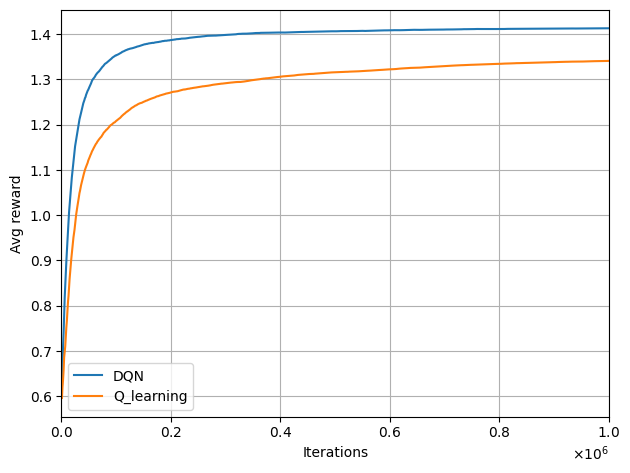
\includegraphics[scale=0.5]{converged}
    \label{fig:converged}
\end{figure}

\subsection{So sánh với chiến lược phòng thủ ''tham lam'' không sử dụng DRL.}
Ở đây, chúng ta thực hiện so sánh giữa việc sử dụng phương án DQN được đề xuất và chiến lược phòng thủ cố định ''tham lam'' được mô tả như sau: (i) Khi
UAV gây nhiễu không tấn công kênh truyền, máy phát sẽ phát chủ động gói tin đến máy thu, (ii) Khi UAV gây nhiễu tấn công kênh truyền, máy phát sẽ tận dụng
sóng nhiễu từ UAV để thu năng lượng hoặc tán xạ ngược đan xen nhau theo một chu kì cố định - máy phát sẽ tiến hành thu năng lượng từ sóng nhiễu sau mỗi chu kì
$T_\text{harvest} = 5$ đơn vị thời gian, thời gian còn lại máy phát sẽ tiến hành tán xạ ngược sóng nhiễu để truyền dữ liệu đến máy thu. Ta gọi chiến lược này
là chiến lược phòng thủ cố định ''tham lam''. Với phương án sử dụng DQN được đề xuất, em thực hiện $4 \times 10^4$ lần lặp để tìm ra chiến lược tối ưu cho máy
phát và sau đó so sánh hiệu quả với chiến lược tham lam đã nêu ở trên.

\begin{enumerate}
    \item[\textbf{a}.] \textbf{Đánh giá hiệu quả khi thay đổi công suất nhiễu.}
    \begin{figure}{So sánh thông lượng trung bình giữa DQN và Greedy $P_\text{avg}$ thay đổi.}
        \centering
        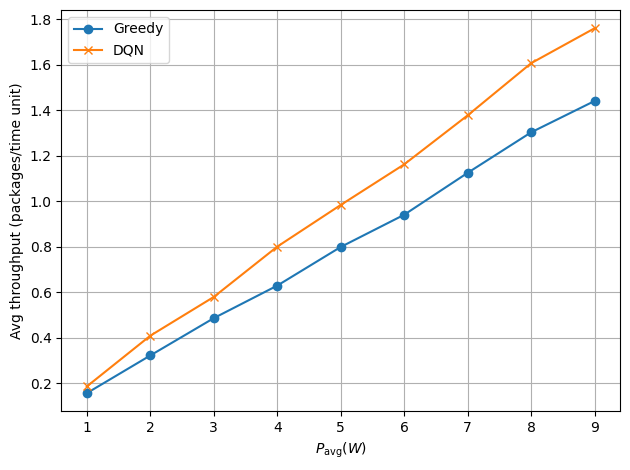
\includegraphics[scale=0.5]{p_avg_throughput}
        \label{fig:p_avg_throughput}
    \end{figure}
    \begin{figure}{So sánh số gói tin mất mát giữa DQN và Greedy $P_\text{avg}$ thay đổi.}
        \centering
        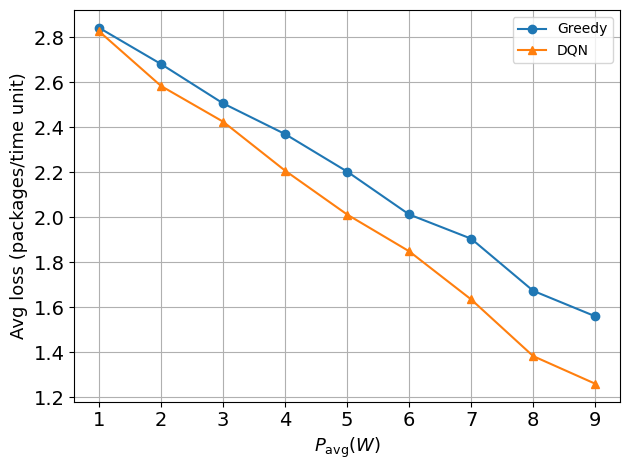
\includegraphics[scale=0.5]{p_avg_loss}
        \label{fig:p_avg_loss}
    \end{figure}
    \begin{figure}{So sánh PDR giữa DQN và Greedy $P_\text{avg}$ thay đổi.}
        \centering
        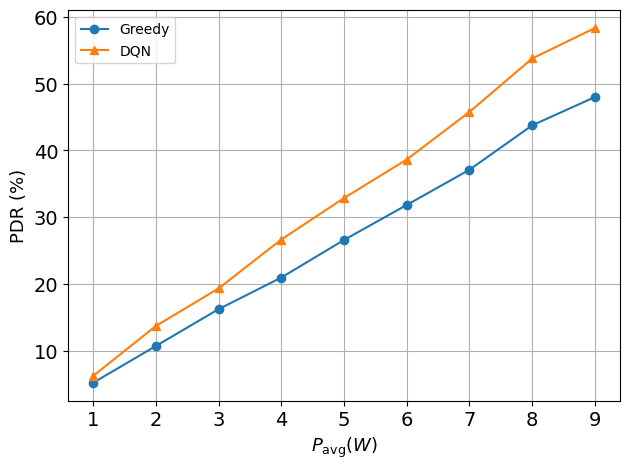
\includegraphics[scale=0.5]{p_avg_pdr}
        \label{fig:p_avg_pdr}
    \end{figure}

    Trong Hình 4.2, Hình 4.3, Hình 4.4, ta thực hiện thay đổi công suất phát của máy gây nhiễu, dễ nhận thấy khi công suất gây nhiễu tăng lên, tức là khả năng 
    máy gây nhiễu tấn công kênh truyền với mức năng lượng lớn dẫn đến khả năng tán xạ ngược sóng nhiễu và khả năng thu năng lượng từ sóng nhiễu cũng tăng lên ở 
    cả 2 phương án. Điều này đã làm cải thiện hiệu năng của hệ thống (thông lượng tăng, số gói tin mất mát giảm và tỉ lệ truyền thành công cao hơn). Tuy nhiên 
    với phương án đề xuất sử dụng học tăng cường sâu, đã giúp máy thu thích ứng được với sự bất định của môi trường nhiễu, với chiến lược tấn công dẫn đến tốc độ 
    cải thiện hiệu năng hệ thống của phương án đề xuất là cao hơn so với phương án sử dụng chiến lược “tham lam” cố định ở trên. Khi công suất trung bình của máy 
    gây nhiễu thấp, dễ nhận thấy 2 phương án có hiệu suất khá tương đồng, tuy nhiên khi công suất nhiễu trung bình càng tăng lên, sự hiệu quả của phương án đề xuất 
    càng thấy rõ.

    \item[\textbf{b}.] \textbf{Đánh giá hiệu quả khi thay đổi số gói tin có thể phát chủ động $\hat{d}_t$.}
    
    Thử nghiệm được thực hiện với công suất nhiễu $P_\text{avg} = 7W$, trong thử nghiệm ở Hình 4.5, Hình 4.6, Hình 4.7 này ta thực hiện thay đổi số gói tin tối đa mà máy phát
    có thể phát chủ động đến máy thu.

    \begin{figure}{So sánh thông lượng trung bình giữa DQN và Greedy $\hat{d}_t$ thay đổi.}
        \centering
        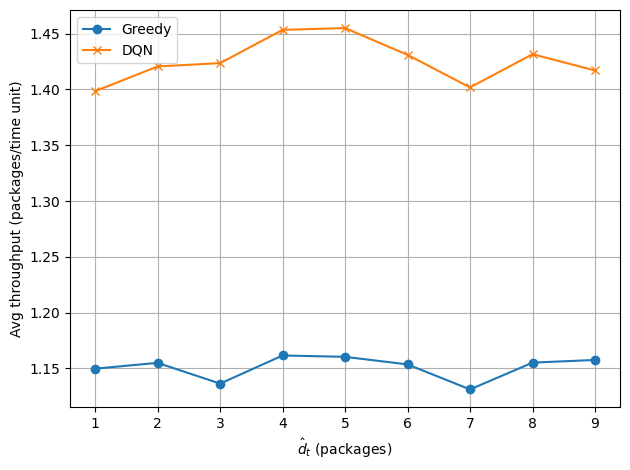
\includegraphics[scale=0.5]{dt_throughput}
        \label{fig:dt_throughput}
    \end{figure}
    \begin{figure}{So sánh số gói tin mất mát giữa DQN và Greedy $\hat{d}_t$ thay đổi.}
        \centering
        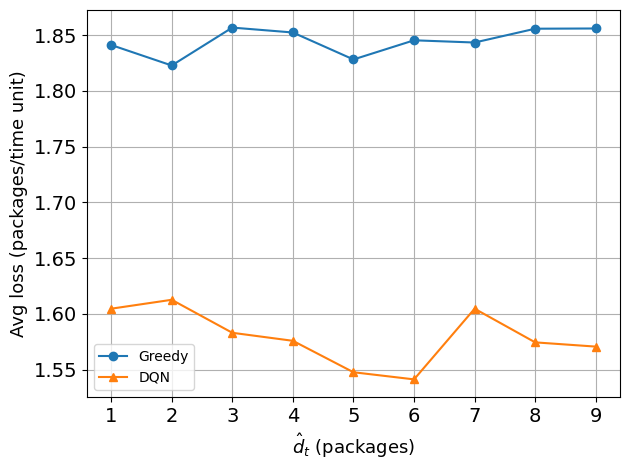
\includegraphics[scale=0.5]{dt_loss}
        \label{fig:dt_loss}
    \end{figure}
    \begin{figure}{So sánh PDR giữa DQN và Greedy $\hat{d}_t$ thay đổi.}
        \centering
        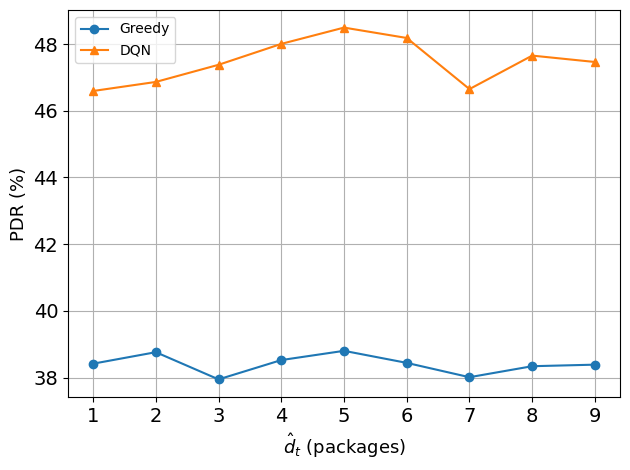
\includegraphics[scale=0.5]{dt_pdr}
        \label{fig:dt_pdr}
    \end{figure}

    \item[\textbf{c}.] \textbf{Đánh giá hiệu quả khi thay đổi chu kì thu năng lượng $T_\text{harvest}$ của máy thu trong phương án sử dụng chiến lược phòng thủ cố định “tham lam”.}
    
    Trong mô phỏng Hình 4.8, Hình 4.9, Hình 4.10 , công suất nhiễu trung bình trong mô phỏng này $P_\text{avg} = 7W$, ta thấy được việc thay đổi chu kì thu năng lượng trong 
    phương án phòng thủ tham lam khiến cho hiệu suất hệ thống thay đổi rõ rệt. Dễ thấy trong trường hợp này,  khi công suất nhiễu cao, cơ hội để máy phát có thể phát 
    chủ động không nhiều dẫn đến chiến lược phòng thủ “tham lam” chủ yếu sẽ truyền gói tin thông qua kĩ thuật tán xạ ngược, điều này khiến cho nếu chu kì thu năng lượng 
    của chiến lược “tham lam” càng lớn (càng ít thực hiện thu năng lượng hơn) sẽ khiến cho thông lượng, số gói tin bị mất và tỉ lệ gói tin thành công tăng nhanh, tuy nhiên
    khi chu kì thu năng lượng tăng đến giá trị 5 đơn vị thời gian thì hiệu quả của hệ thống với chiến lược tham lam gần như không thay đổi nhiều, do lúc này máy phát chủ yếu 
    lựa chọn tán xạ ngược thay vì thu năng lượng để chờ cơ hội phát chủ động, dẫn đến hiệu quả tán xạ ngược đã đạt gần giá trị tối ưu, khiến cho hiệu quả của hệ thống gần 
    như ổn định. Tuy nhiên vẫn chưa thể đạt đến hiệu quả như phương án đề xuất sử dụng DQN mang lại.
    \begin{figure}{So sánh thông lượng trung bình giữa DQN và Greedy $T_\text{harvest}$ thay đổi.}
        \centering
        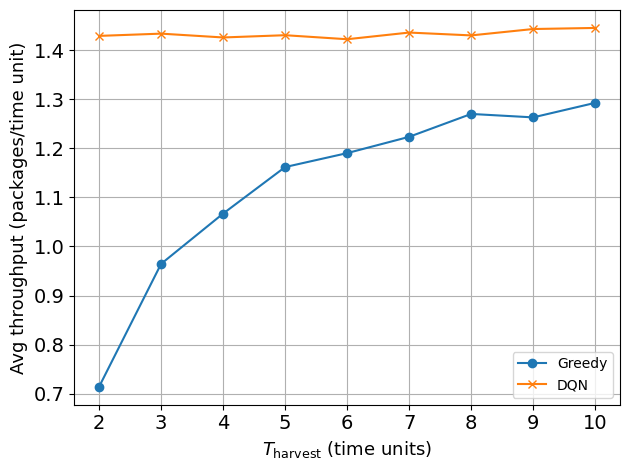
\includegraphics[scale=0.5]{t_harvest_throughput.png}
        \label{fig:t_throughput}
    \end{figure}
    \begin{figure}{So sánh số gói tin mất mát giữa DQN và Greedy $T_\text{harvest}$ thay đổi.}
        \centering
        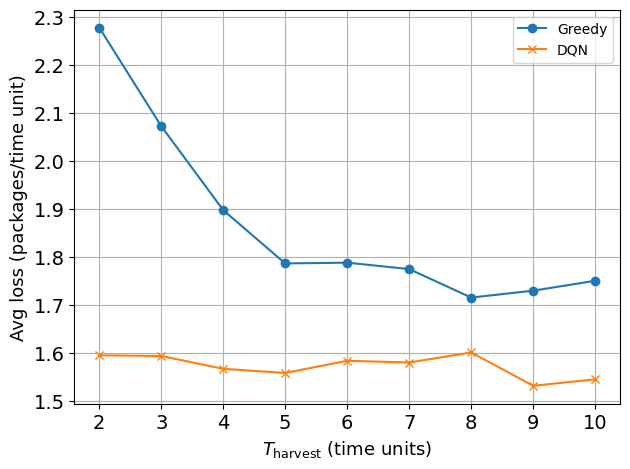
\includegraphics[scale=0.5]{t_harvest_loss.png}
        \label{fig:t_loss}
    \end{figure}
    \begin{figure}{So sánh PDR giữa DQN và Greedy $T_\text{harvest}$ thay đổi.}
        \centering
        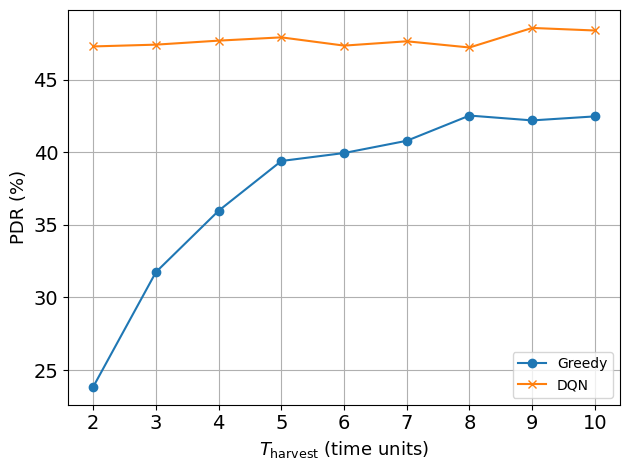
\includegraphics[scale=0.5]{t_harvest_pdr.png}
        \label{fig:t_pdr}
    \end{figure}

\end{enumerate}
% Chapter 5
\chapter{Kết luận}
Trong đồ án này, em đã đề xuất một phương pháp chống nhiễu cho hệ thống truyền thông không dây để chống lại cuộc tấn công từ thiết bị gây nhiễu gắn trên máy bay không người lái UAV.
Máy phát trong trường hợp này có thể tận dụng sóng nhiễu từ thiết bị tấn công để thu năng lượng để phục vụ hoạt động truyền gói tin chủ động khi không bị tấn công, hoặc điều chỉnh tốc
độ phát thích hợp, hoặc tận dụng sóng nhiễu để tán xạ ngược gói tin đến máy thu. Dựa trên việc xây dựng mô hình hệ thống truyền thông này như một bài toán MDP, em đã đã sử dụng các
thuật toán học tăng cường như
Q-learning và DQN để giúp máy phát tìm ra được chiến lược phòng thủ phù hợp trước cuộc tấn công gây nhiễu, qua đó tối đa hoá thông lượng trung bình của hệ thống, giảm số gói tin bị mất mát trên đường truyền.
Kết quả mô phỏng đã chỉ ra rằng, với việc sử dụng các thuật toán học tăng cường, thông lượng của hệ thống cũng như số gói tin mất mát và tỉ lệ truyền gói tin thành công đều tăng lên rõ
rệt so với một chiến lược truyền tin tham lam không sử dụng thuật toán học tăng cường. Qua đó giúp hệ thống không những có khả năng chống lại, mà còn tận dụng được cuộc tấn công gây nhiễu
để thực hiện nhiệm vụ truyền thông tin của mình và giảm thiểu thiệt hại của cuộc tấn công gây nhiễu.

% Tài liệu tham khảo
\begin{thebibliography}{9}
\begin{bibsection}{Tiếng Anh}
    % Book
    \bibitem{hoang2023deep}
    Hoang, D.T. and Van Huynh, N. and Nguyen, D.N. and Hossain, E. and Niyato, D.
    \textit{Deep Reinforcement Learning for Wireless Communications and Networking: Theory, Applications and Implementation},
    \textit{Wiley}, 2023, pp. 37-163.
    \bibitem{Sutton}
    R. S. Sutton and A. G. Barto, Reinforcement learning: An introduction.
    MIT Press, 2018.
    % Paper
    \bibitem{Hossein22}
    Pirayesh, Hossein and Zeng, Huacheng
    ''Jamming Attacks and Anti-Jamming Strategies in Wireless Networks: A Comprehensive Survey'',
    \textit{IEEE Communications Surveys \& Tutorials},
    vol. 24, no. 2,
    pp. 767-809

    \bibitem{Vadlamani16}
    Satish Vadlamani,Burak Eksioglu,Hugh Medal,Apurba Nandi
    ''Jamming attacks on wireless networks: A taxonomic survey'',
    \textit{International Journal of Production Economics},
    vol. 172,
    2016,
    pp. 76-94

    \bibitem{Xu2005}
    Xu, Wenyuan and Trappe, Wade and Zhang, Yanyong and Wood, Timothy
    ''The feasibility of launching and detecting jamming attacks in wireless networks'',
    \textit{Association for Computing Machinery},
    2005,
    pp. 46–57
    \bibitem{Vincent}
    Ambient Backscatter: Wireless Communication Out of Thin Air
    \bibitem{Ning_Gao}
    Anti-Intelligent UAV Jamming Strategy via Deep Q-Networks
    \bibitem{jam_me}
    “Jam Me If You Can”: Defeating Jammer with Deep Dueling Neural Network Architecture and Ambient Backscattering Augmented Communications
\end{bibsection}
\end{thebibliography}
\end{document}